实际项目中使用编程语言,是学习语言的一个步骤。有时,本书中的简单例子可能采用不同的方法,或者在实际程序中面临许多困难。理论需要与实践相结合。与学习语法、解决书本上的问题或理解书本上一些简单的例子不同,当创建实际的应用程序时,我们会面临一系列不同的挑战,有时书籍缺乏理论来支持实际问题。 \par
我们将尝试梳理C++实际编程的知识,这将帮助你更好地处理实际的应用程序。复杂的项目需要大量的思考和设计。有时候,因为开发者在开发之初做出了糟糕的设计选择,所以需要从头开始重写项目。本章描述了软件的设计过程。读者将了解为项目构建架构的步骤。\par
本章中,我们将了解以下内容: \par

\begin{itemize}
	\item 了解项目开发周期
	\item 设计模式及应用
	\item 领域驱动设计
	\item 设计一个Amazon的克隆版本作为一个真实项目
\end{itemize}

\noindent\textbf{}\ \par
\textbf{编译器要求} \ \par
g++编译器需要添加编译选项 \texttt{-std=c++2a} 来编译本章的代码。可以从这里获取本章的源码文件:https:/​/github.​com/PacktPublishing/Expert-CPP \par

\noindent\textbf{}\ \par
\textbf{项目开发周期} \ \par
当处理一个问题时,应该仔细考虑需求分析的过程。项目开发中最大的错误之一是,在开始编码时没有对问题本身进行彻底的分析。 \par
想象一下这样一个场景,你的任务是创建一个计算器,允许用户对数字进行算术计算的简单工具。假设你奇迹般地按时完成了项目并发布了程序。现在,用户开始使用计算器,他们迟早会发现他们的计算结果不会超过整数的最大值。当他们抱怨这个问题时,就可以准备用可靠的编码来辩解,比如:它是因为在计算中使用了int数据类型。这对于你和你的程序员伙伴来说是完全可以理解的,但是最终用户就是不能接受你的观点。他们想要一个能够对大数字求和的工具,否则,他们根本不会使用你的程序。开始开发下一个版本的计算器时,将使用长数或甚至自定义实现的大数。当你自豪的将第二版程序交付给等待已久的用户时,用户可能会抱怨没有找到数字的对数或指数的功能。这就令人生畏了,因为可能会有越来越多的特性请求和越来越多的抱怨。 \par
虽然这个例子有点简单,但它完全涵盖了现实世界中经常发生的事情。即使开发者实现了程序的所有特性,并且正在考虑休假,用户也会开始抱怨程序中的错误。结果表明,有几种情况下,计算器的行为异常,没有给出或给出了错误的结果。迟早,您会意识到,在将程序发布给大众之前,需要的是适当的测试。 \par
我们将涉及在实际项目中工作时应该考虑的主题。当开始一个新项目时,应该考虑以下步骤: \par

\begin{enumerate}
	\item 需求收集和分析
	\item 创建规范
	\item 设计和测试计划
	\item 编码
	\item 测试和稳定性
	\item 发布和维护
\end{enumerate}

前面的步骤并不是针对每个项目都固定的,应该认为是每个软件开发团队为了实现成功的产品发布而应该完成的最低要求。现实中,大部分的步骤都被省略了,因为在IT领域的每个人都缺乏一件东西——时间。但是,强烈建议遵循上述步骤,因为从长远来看,它会节省更多的时间。 \par

\noindent\textbf{}\ \par
\textbf{需求收集和分析} \ \par
这是创建稳定产品的最关键的一步。开发者不能按时完成任务,或在代码中留下大量bug的一个最普遍的原因是缺乏对项目的完整理解。 \par
领域知识是如此重要,不应该被忽略。在任何情况下,你可能会很幸运地开发与你非常了解的东西相关的项目。然而,你应该考虑到不是每个人都像你一样幸运。 \par
假设您正在进行一个项目,该项目将自动分析和报告某个公司的股票交易信息。现在想象一下,你对股票和股票交易一无所知。你不知道熊市或牛市,交易的局限性等等。你将如何成功地完成这个项目? \par
即使您了解股票市场和交易,您也可能不知道您的下一个大型项目域。如果你的任务是设计和执行(有或没有团队)一个控制城市气象站的项目,那该怎么办?当你开始这个项目时,你首先要做什么? \par
你肯定应该从需求收集和分析开始。这只是一个涉及到与客户沟通和问很多关于项目的问题的过程。如果你在一家产品公司工作,而不是与任何客户打交道,那么项目经理就应该视为客户。即使这个项目是你的想法,你是独自工作,你也应该把自己当成客户,尽管这听起来可能有些荒谬,但你应该问自己很多问题(关于这个项目)。 \par
假设我们将征服电子商务,并希望发布一种产品,最终将在自己的业务领域击败市场大鳄。受欢迎和成功的电子商务市场有亚马逊、eBay、阿里巴巴等。我们应该把这个问题表述为,编写自己的Amazon版本。我们应该如何收集这个项目的需求? \par
首先,我们应该列出所有我们应该实现的功能,然后我们将优先级排序。例如,对于Amazon的项目,我们可能会得到以下特性列表: \par

\begin{itemize}
	\item 创建产品
	\item 展示产品
	\item 购买产品
	\item 修改产品的信息
	\item 删除产品
	\item 通过名称、价格范围和重量搜索产品
	\item 每隔一段时间通过电子邮件告知用户产品的可用性
\end{itemize}

应该尽可能详细地描述功能,这将为开发人员解决问题。例如,创建产品应该由项目管理员或任何用户完成。如果用户可以创建产品,则应该有限制。用户可能会错误地在我们的系统中创建数百个产品,以增加他们唯一产品的可见性。 \par
与客户沟通的过程中,应陈述、讨论和最终确定细节。如果项目中只有你一人,并且你是项目的客户,那么交流就是你自己对项目需求进行思考的过程。 \par
当完成获取需求时,我们建议对每个特性进行优先级排序,并将它们分为以下类别之一: \par

\begin{itemize}
	\item 刚性要求
	\item 应该拥有
	\item 最好具有
\end{itemize}

进一步思考并对上述特性进行分类后,我们可以得出以下列表: \par

\begin{itemize}
	\item 创建产品[刚性要求]
	\item 展示产品[刚性要求]
	\item 购买产品[刚性要求]
	\item 修改产品的信息[应该拥有]
	\item 删除产品[刚性要求]
	\item 通过名称搜索产品[刚性要求]
	\item 通过价格范围搜索产品[应该拥有]
	\item 通过重量搜索产品[最好具有]
	\item 每隔一段时间通过电子邮件告知用户产品的可用性[最好具有]
\end{itemize}

分类会让你大致知道从哪里开始。开发者是贪婪的人,他们想为自己的产品实现所有可能的功能,这肯定会导致失败。你应该先从最基本的功能开始——这就是为什么会有一些很好的功能。 \par

\noindent\textbf{}\ \par
\textbf{创建规范} \ \par
并不是每个人都喜欢创建规范说明。大多数开发者讨厌这个步骤,因为它不是编码,而是编写文档。 \par
收集项目需求之后,应该创建一个文档,其中包括描述项目的每个细节。该规范有许多名称和类型。可以称为项目需求文档(PRD)、功能规范、开发规范等。认真的开发者和认真的团队根据需求分析生成一个PRD,下一步是创建功能规范和开发规范等。我们将所有的文档组合在一个名为规范创建的步骤中。 \par
你和你的团队可以决定是否需要前面提到的任何子文档,用可视化的产品表示比用文本文档更好。无论文档采用何种形式,它都应该仔细地表示在需求收集步骤中取得的成果。为了对此有一个基本的理解,让我们尝试着记录一些之前收集到的特性(我们把这个项目称为\texttt{the platform}) \par

\begin{itemize}
	\item 创建一个产品。拥有管理员权限的平台用户可以创建产品。
	\item 平台必须允许创建具有定义权限的用户。此时,应该有两种类型的用户,即普通用户和管理员用户。
	\item 任何使用该平台的用户都必须能够看到可用产品的列表。
	\item 产品应该有图片、价格、名称、重量和描述。
	\item 要购买一个产品,用户提供他们的卡的详细信息来兑现和产品发货的详细信息。
	\item 每个注册用户应提供送货地址、信用卡详细信息和电子邮件帐户。
\end{itemize}

列表可能很长,实际上也应该很长,因为列表越长,开发人员对项目的理解就越多。 \par

\noindent\textbf{}\ \par
\textbf{设计和测试计划} \ \par
尽管我们坚持认为需求收集步骤是软件开发中最重要的步骤,但是设计和测试计划也是同样重要的步骤。尽管励志格言坚持认为没有什么是不可能的,但开发者们确信至少有一件事是不可能的,那就是不先设计就成功地完成一个项目。 \par
设计的过程是最有趣的步骤,它迫使我们思考、描绘、再思考、清除一切,然后重新开始。项目的许多特性是在设计时发现的。设计一个项目,应该从头开始。首先,列出以某种方式与项目相关的所有实体和过程。对于Amazon克隆的例子,我们可以列出以下过程: \par

\begin{itemize}
	\item 用户
	\item 注册和授权
	\item 产品
	\item 交易
	\item 仓库(包含产品)
	\item 装运
\end{itemize}

这是一个高层次的设计——贯穿最终设计的起点。本章中,我们将主要集中在项目的设计上。 \par

\noindent\textbf{}\ \par
\textbf{需求分解} \ \par
列出关键步骤和流程之后,我们将它们分解为更详细的步骤,这些步骤稍后将转换为类。最好是画出项目的设计草图,只需绘制包含实体名称的矩形,如果以某种方式连接在一起或是同一过程的一部分,则用箭头连接它们,这是一个更好的理解项目必要的一步。例如,请看下面的图表: \par

\begin{center}
	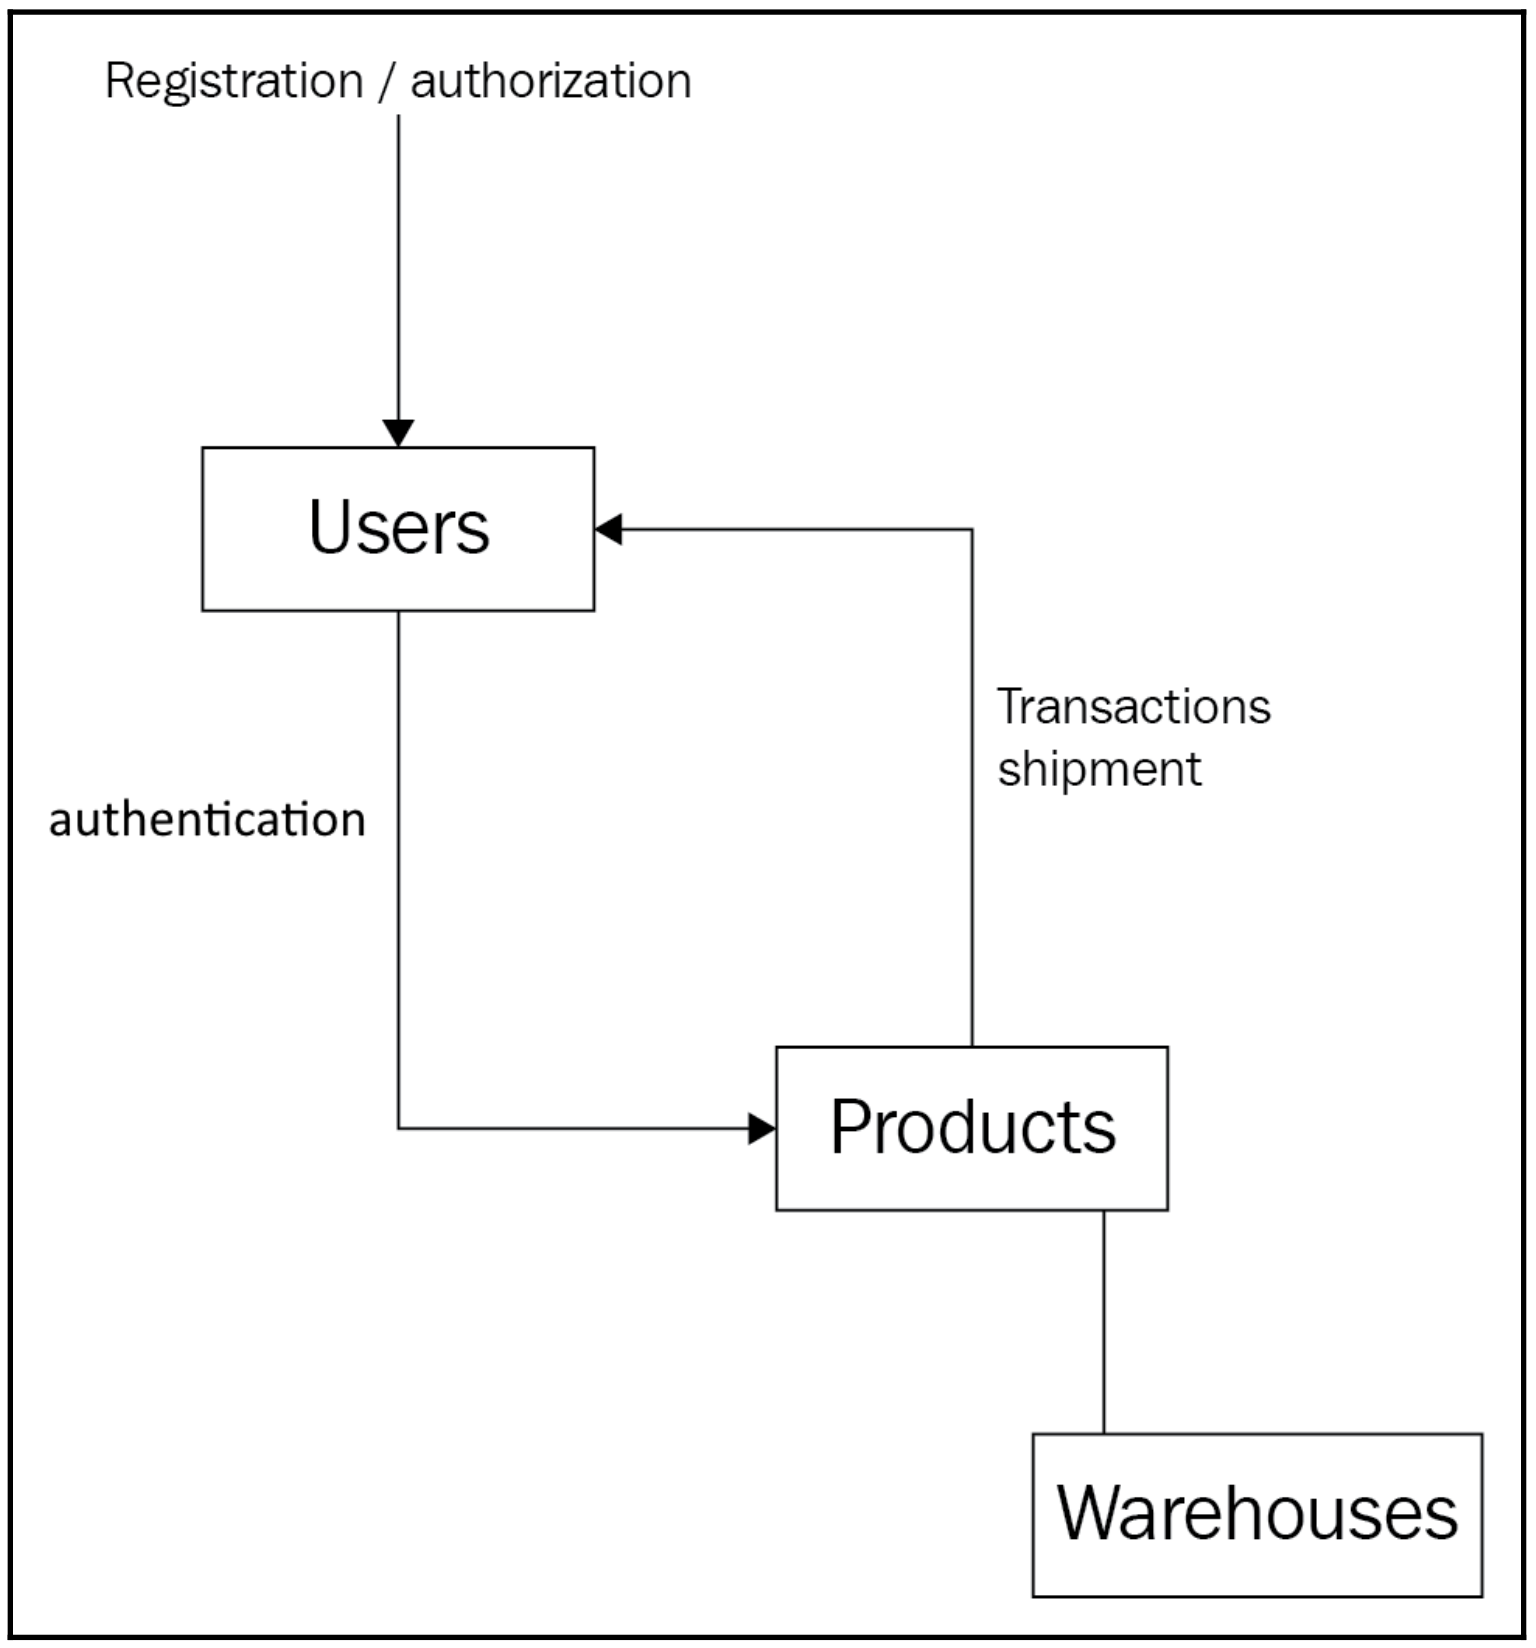
\includegraphics[width=0.6\textwidth]{content/Section-2/Chapter-10/1}
\end{center}

把实体和过程分解成类,它们之间的相互交流就是一门艺术,需要耐心和一致性。例如,我们尝试添加用户实体的详细信息。如创建规范步骤中所述,注册用户应该提供送货地址、电子邮件地址和信用卡详细信息。让我们画一个表示用户的类图: \par

\begin{center}
	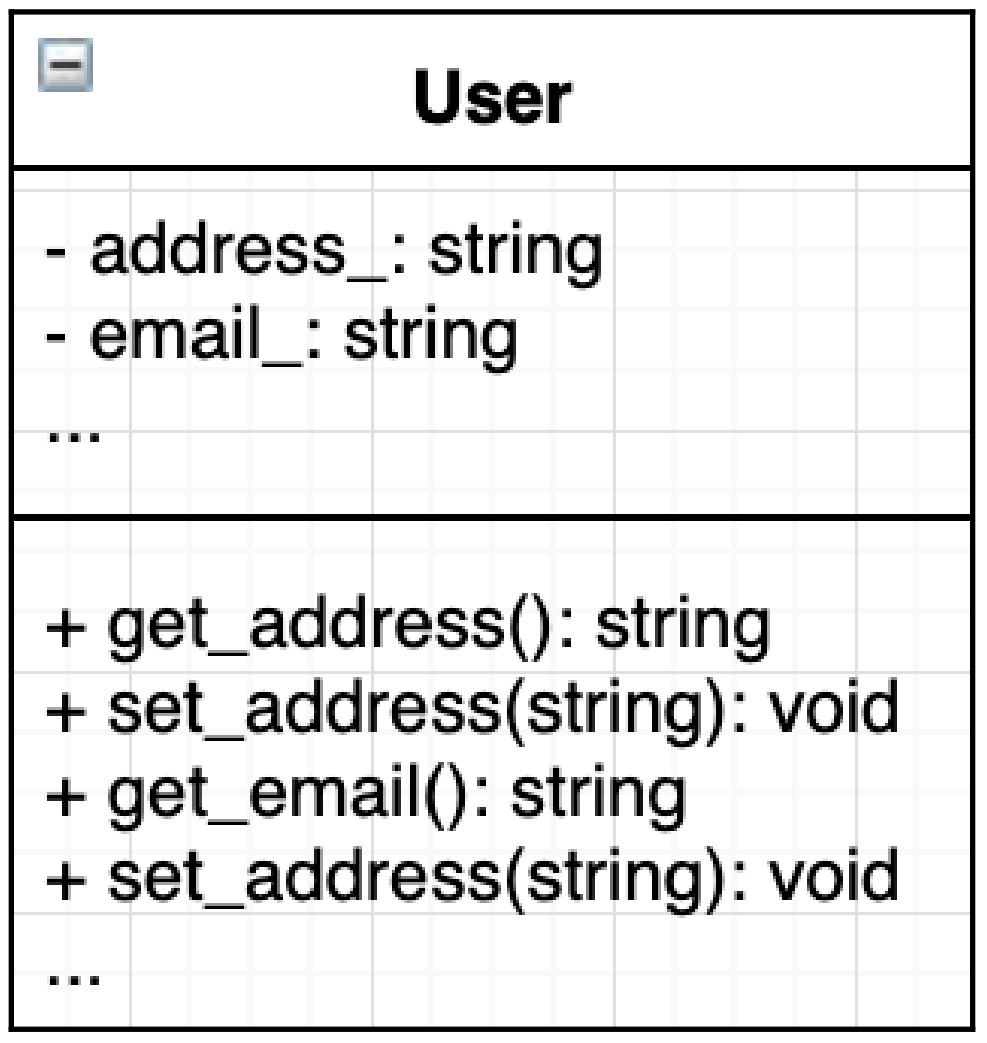
\includegraphics[width=0.4\textwidth]{content/Section-2/Chapter-10/2}
\end{center}

有一个有趣的问题:我们如何处理复杂类型?例如,用户的投递地址是复杂类型。它不可能只是字符串,因为我们可能需要根据用户的送货地址进行排序,以实现最佳的发货顺序。如果用户的送货地址与包含购买产品的仓库地址在不同的国家,那么货运公司可能会让我们(或用户)花费一大笔钱。这是一个很好的场景,它引入了一个新的问题,并更新了我们对项目的理解。当用户订购的产品分配到离用户很远的仓库时,我们应该处理这种情况。如果我们有很多仓库,我们应该选择一个距离用户最近的。这些问题不能马上得到具体的回答,但这可以保证项目的高质量。否则,这些问题就会在编码过程中出现,我们困在这些问题上的时间,就要比我们想象的要长。 \par
现在,如何将用户地址存储在User类中?一个简单的std::string就可以了,如下面的例子所示: \par

\begin{lstlisting}[caption={}]
class User
{
public:
	// code omitted for brevity
private:
	std::string address_;
	// code omitted for brevity
};
\end{lstlisting}

就其组件而言,地址是一个复杂的对象。地址可以包含国家名称、国家代码、城市名称和街道名称,甚至还可以包含纬度和经度。如果您需要找到离用户最近的仓库,那么越详细越好。制作更多类型,让开发者的设计更直观,这完全没有问题。例如,下面的结构体可能很适合描述用户的地址: \par

\begin{lstlisting}[caption={}]
struct Address
{
	std::string country;
	std::string city;
	std::string street;
	float latitude{};
	float longitude{};
};
\end{lstlisting}

现在,存储用户地址变得更加简单: \par

\begin{lstlisting}[caption={}]
class User
{
	// code omitted for brevity
	Address address_;
};
\end{lstlisting}

设计项目的过程,可能需要有几个步骤重申项目需求。用前面的步骤澄清设计步骤之后,我们可以继续将项目分解为更小的组件,最好也都创建交互图。 \par
如下所示的交互图,将描述用户购买产品时所做的交易等操作: \par

\begin{center}
	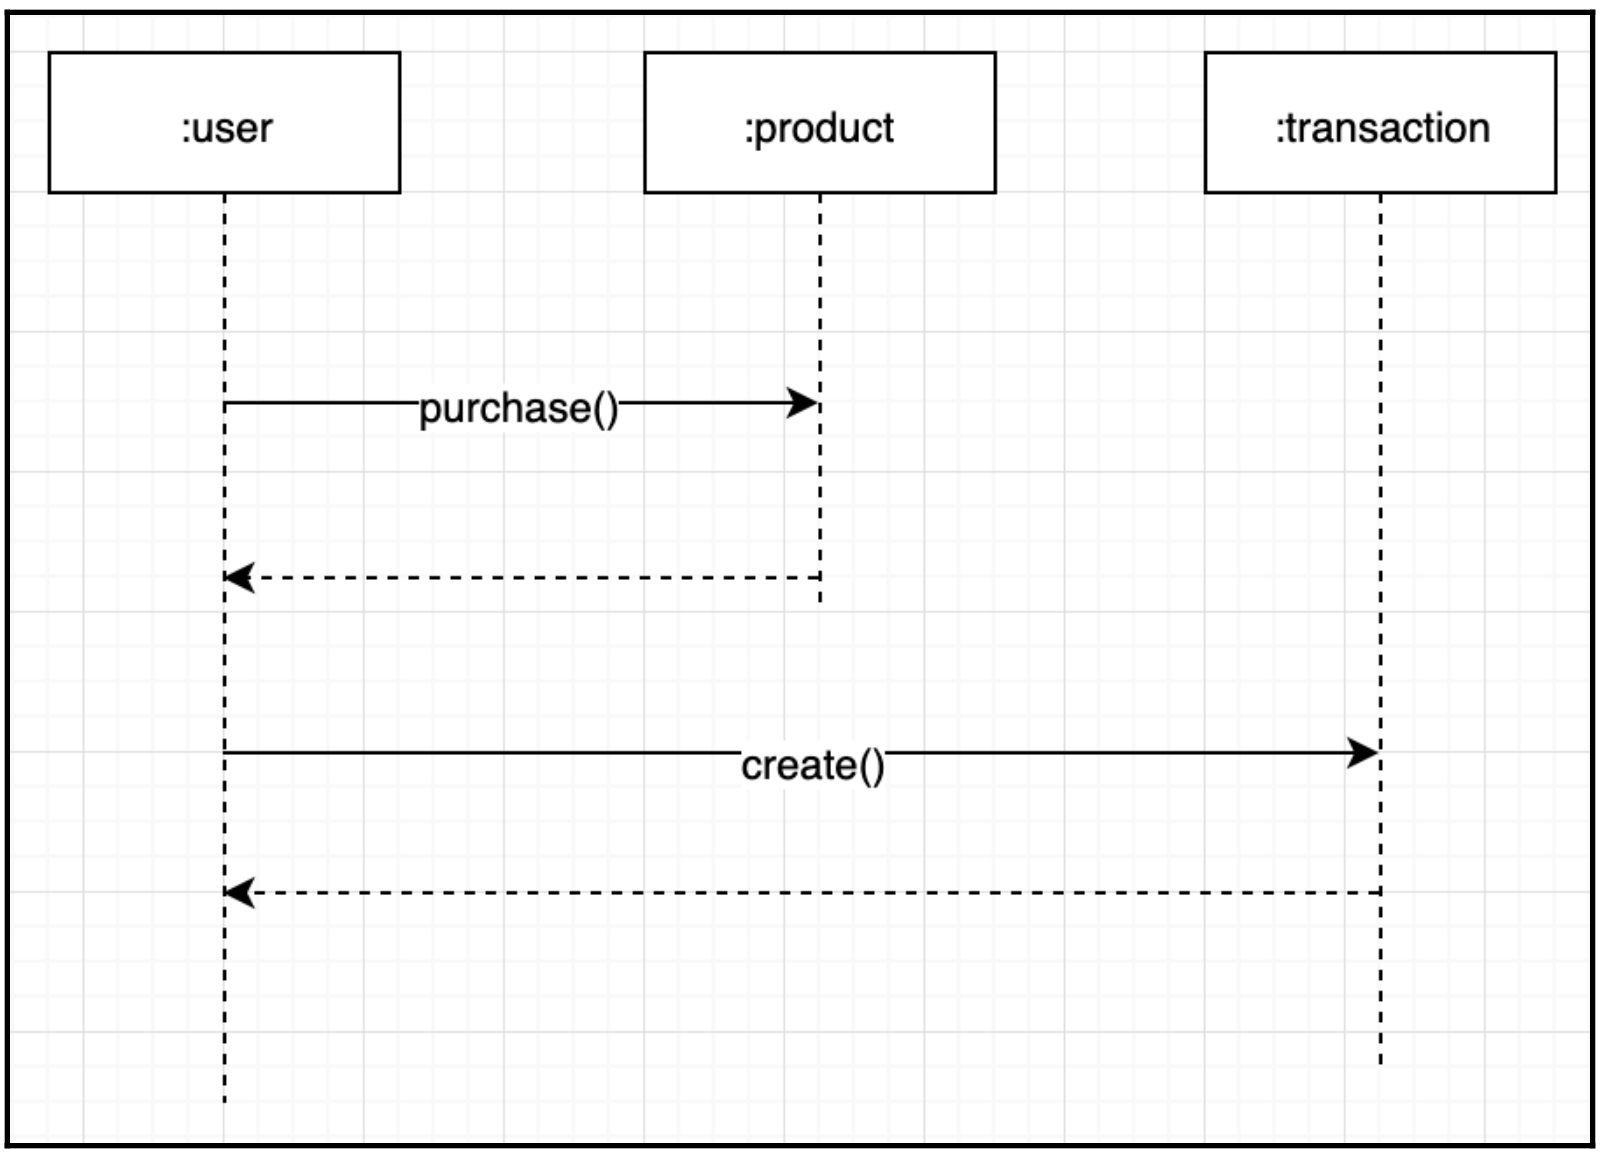
\includegraphics[width=0.8\textwidth]{content/Section-2/Chapter-10/3}
\end{center}

测试计划也可以认为是设计的一部分,包括如何测试最终应用程序的计划,例如:在此之前的步骤包括一个地址的概念,地址可以包含国家、城市等。正确的测试应该包括,检查是否可以在用户地址中成功设置国家。虽然测试计划通常不认为是开发者的任务,但对项目来说,它是一种很好的实践。在设计项目时,适当的测试计划将产生更多有用的信息。大多数输入数据处理和安全检查都在测试计划中发现,例如:在进行需求分析或编写功能规范时,对用户名或电子邮件地址设置严格的限制可能并不适用。测试计划会关注这样的场景,并迫使开发人员进行数据检查。然而,大多数开发人员并没有耐心做这些,而是直接进入项目开发的下一个步骤——编码。 \par

\noindent\textbf{}\ \par
\textbf{编码} \ \par
如前所述,编码并不是项目开发的唯一。编码之前,应该通过规范中的需求来仔细设计项目。在完成前面的项目开发步骤后,编码将变得容易和高效。 \par
一些团队实践测试驱动开发(TDD),这是产生更稳定项目的好方法。TDD的主要概念是在项目实现之前编写测试。这是开发者定义项目需求和回答开发过程中出现问题的好方法。 \par
假设我们正在为User类实现setter。User对象包含电子邮件字段,所以应该也有一个set\underline{ }email()方法,如下所示: \par

\begin{lstlisting}[caption={}]
class User
{
public:
	// code omitted for brevity
	void set_email(const std::string&);
private:
	// code omitted for brevity
	std::string email_;
};
\end{lstlisting}

TDD方法建议在实现set\underline{ }email()之前,为set\underline{ }email()方法编写一个测试函数。测试函数如下所示: \par

\begin{lstlisting}[caption={}]
void test_set_email()
{
	std::string valid_email = "valid@email.com";
	std::string invalid_email = "112%$";
	User u;
	u.set_email(valid_email);
	u.set_email(invalid_email);
}
\end{lstlisting}

前面的代码中,我们声明了两个字符串变量,其中一个包含无效的电子邮件地址值。在运行测试函数之前,我们就知道在无效数据输入的情况下,set\underline{ }email()方法应该以某种方式做出反应。常见的方法是抛出一个提示无效输入的异常。可以忽略set\underline{ }email实现中的无效输入,并返回一个布尔值,指示操作的成功。错误处理应该在项目中保持一致,并得到所有团队成员的同意。考虑一下抛出异常,测试函数在处理无效值时应该期待异常。 \par
上面的代码应该重写,如下所示: \par

\begin{lstlisting}[caption={}]
void test_set_email()
{
	std::string valid_email = "valid@email.com";
	std::string invalid_email = "112%$";
	
	User u;
	u.set_email(valid_email);
	if (u.get_email() == valid_email) {
		std::cout << "Success: valid email has been set successfully" <<
		std::endl;
	} else {
		std::cout << "Fail: valid email has not been set" << std::endl;
	}

	try {
		u.set_email(invalid_email);
		std::cerr << "Fail: invalid email has not been rejected" << std::endl;
	} catch (std::exception& e) {
		std::cout << "Success: invalid email rejected" << std::endl;
	}
}
\end{lstlisting}

测试功能似乎已经完成。无论何时运行测试函数,都会输出set\underline{ }email()的当前状态。即使我们还没有实现set\underline{ }email()函数,相应的测试函数也是实现细节的一大步。现在有了函数实现,所以了解了如何对有效和无效的数据输入作出反应。我们可以添加更多类型的数据,以确保set\underline{ }email()方法在实现完成时进行彻底的测试。例如,可以用空字符串和长字符串来测试它。 \par
下面是set\underline{ }email()方法的初始实现: \par

\begin{lstlisting}[caption={}]
#include <regex>
#include <stdexcept>

void User::set_email(const std::string& email)
{
	if (!std::regex_match(email,
	std::regex("(\\w+)(\\.|_)?(\\w*)@(\\w+)(\\.(\\w+))+")) {
		throw std::invalid_argument("Invalid email");
	}

	this->email_ = email;
}
\end{lstlisting}

初始实现之后,我们应该再次运行我们的测试函数,以确保实现与定义的测试用例一致。 \par

\hspace*{\fill} \\ %插入空行

\includegraphics[width=0.05\textwidth]{images/tip}
为项目编写测试被认为是一种良好的编码实践。有不同类型的测试,比如:单元测试、回归测试、冒烟测试等。开发人员应该支持他们项目的单元测试覆盖率。 \par
\noindent\textbf{}\ \par

编码过程是项目开发生命周期中最混乱的步骤之一。很难估计实现一个类或它的方法需要多长时间,因为大多数问题和困难都出现在编码过程中。本章开头所描述的项目开发生命周期的前面步骤,往往涵盖了这些问题中的大部分,并简化了编码过程。 \par

\noindent\textbf{}\ \par
\textbf{测试和稳定性} \ \par
项目完成后,应该对其进行适当的测试。通常,软件开发公司有质量保证(QA)工程师,他们会一丝不苟地测试项目。 \par
测试阶段验证的问题会转换成分配给开发者的相应任务,问题可能会影响项目的发布。 \par
开发者的基本任务不是立即修复问题,而是找到问题的根本原因。为了简单起见,让我们看一下generate\underline{ }username()函数,它使用随机数结合电子邮件来生成用户名: \par

\begin{lstlisting}[caption={}]
std::string generate_username(const std::string& email)
{
	int num = get_random_number();
	std::string local_part = email.substr(0, email.find('@'));
	return local_part + std::to_string(num);
}
\end{lstlisting}

generate\underline{ }username()函数调用get\underline{ }random\underline{ }number(),将返回的值与电子邮件地址的私有部分结合起来。私有部分是电子邮件地址中@符号之前的部分。 \par
QA工程师报告说,邮件中附在私有部分的数字一直是一样的。例如,对于电子邮件john@gmail.com,生成的用户名是john42,对于amanda@yahoo.com,生成的用户名是amanda42。因此,下一次使用电子邮件amanda@hotmail.com的用户试图在系统中注册时,生成的用户名amanda42与已经存在的用户名冲突。测试人员完全不知道项目的实现细节,所以他们会在用户名生成功能中报告这个问题。虽然您可能已经猜到真正的问题隐藏在get\underline{ }random\underline{ }number()函数中,但总是存在这样的情况,问题修复了,但没找到根本原因。修复问题的错误方法可能会改变generate\underline{ }username()函数的实现。generate\underline{ }random\underline{ }number()函数也可能在其他函数中使用,这反过来会使所有调用get\underline{ }random\underline{ }number()的函数得到错误结果。尽管例子很简单,但深入思考并找到问题背后的真正原因才是至关重要的。 \par

\noindent\textbf{}\ \par
\textbf{发布和维护} \ \par
通过修复所有关键和主要问题,项目稳定之后,就可以发布了。有时候,公司发布的软件打着测试版的标签,这样就有了一个借口,以防用户发现软件漏洞百出。需要注意的是,很少有软件能够完美地工作。在发布之后,会出现更多的问题。因此,当开发人员致力于修复和发布更新时,就会进入维护阶段。 \par
开发者有时开玩笑说,发布和维护是从未实现的步骤。然而,如果花了足够的时间来设计项目,那么发布第一个版本就不会花太多时间。正如我们在前一节已经介绍过的,设计从收集需求开始。之后,我们花时间定义规范,分解它们,分解成更小的组件,编码,测试,最后发布它。作为开发人员,我们对设计和编码阶段更感兴趣。如前所述,一个好的设计选择对进一步的项目开发有很大的影响。现在让我们从整体上仔细看看设计过程。 \par

\noindent\textbf{}\ \par
\textbf{深入设计过程} \ \par
如前所述,在设计电子商务平台时,项目设计从列出一般实体开始,如用户、产品和仓库: \par

\begin{center}
	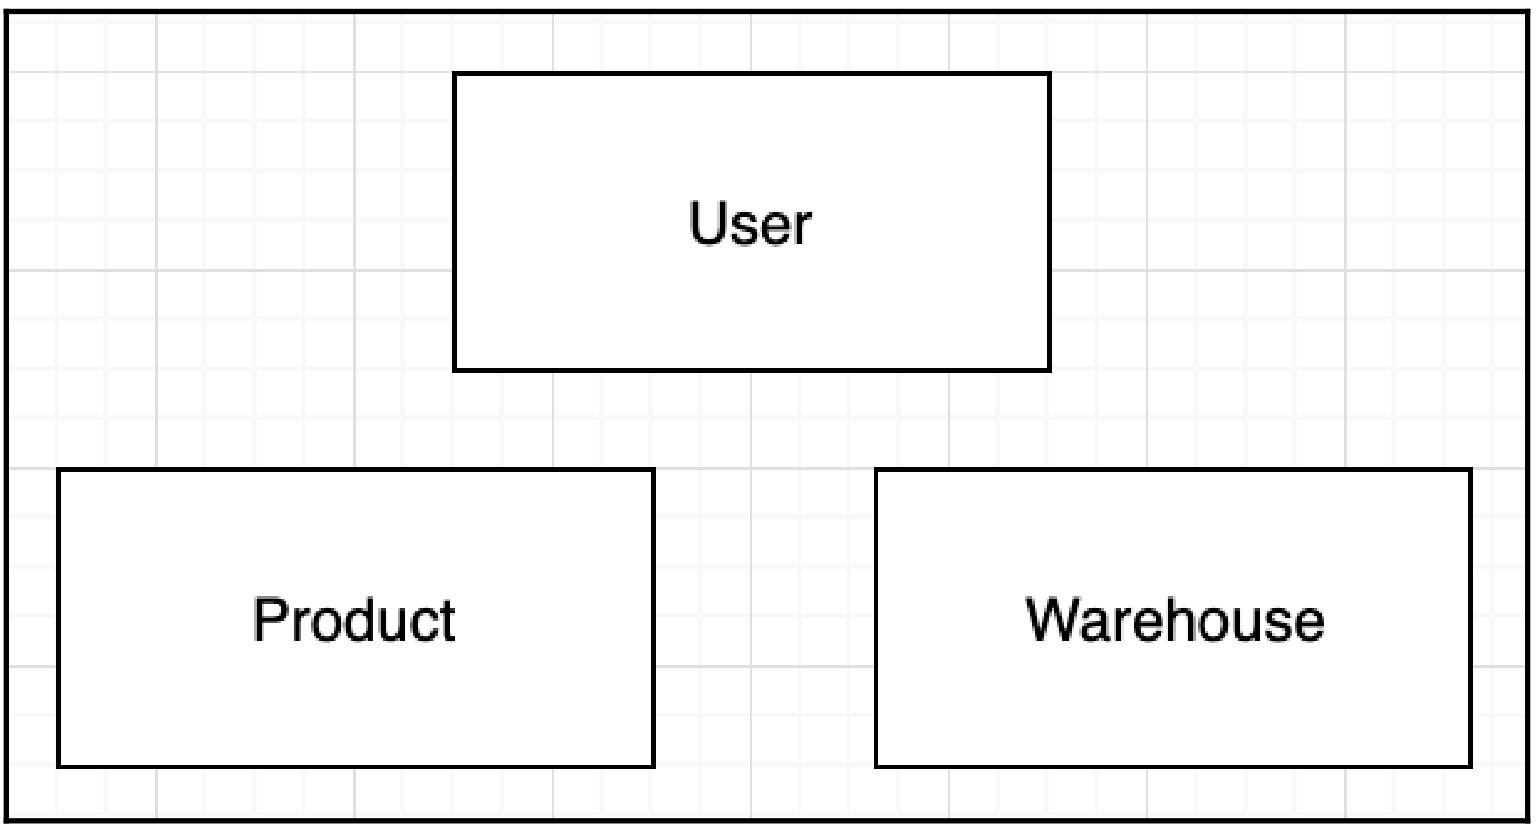
\includegraphics[width=0.8\textwidth]{content/Section-2/Chapter-10/4}
\end{center}

然后我们将每个实体分解成更小的组件。为了让事情更清楚,把每个实体看作一个单独的类。当把一个实体看作一个类时,它在分解方面更有意义。例如,我们将User实体表示为一个类: \par

\begin{lstlisting}[caption={}]
class User
{
public:
	// constructors and assignment operators are omitted for code brevity
	void set_name(const std::string& name);
	std::string get_name() const;
	void set_email(const std::string&);
	std::string get_email() const;
	// more setters and getters are omitted for code brevity
	
private:
	std::string name_;
	std::string email_;
	Address address_;
	int age;
};
\end{lstlisting}

User类的类图如下: \par

\begin{center}
	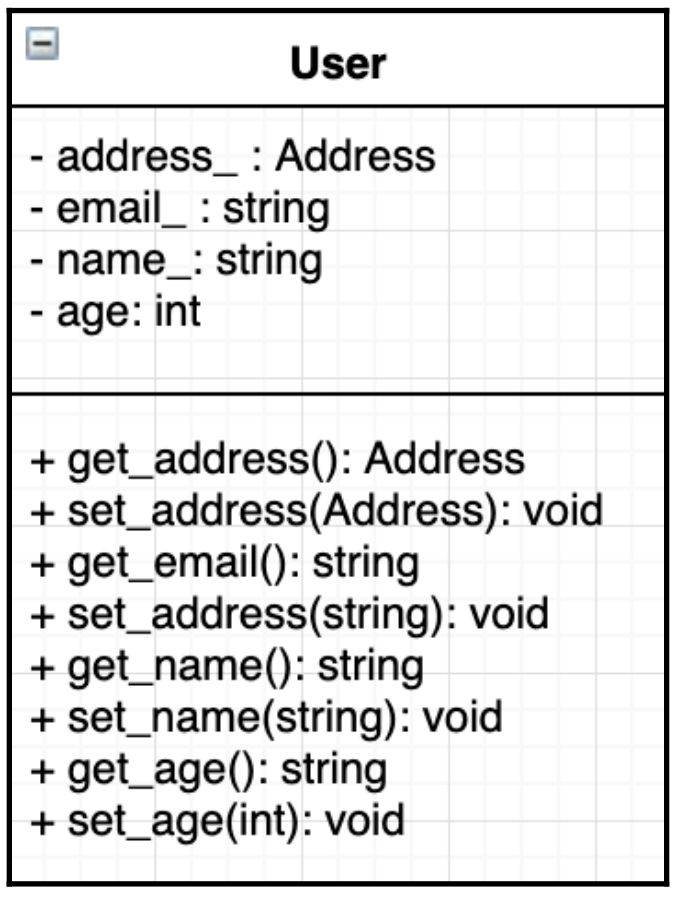
\includegraphics[width=0.4\textwidth]{content/Section-2/Chapter-10/5}
\end{center}

然而,正如我们已经讨论过的,User类的address字段可以表示为一个单独的类型(class或struct,这还不是很重要)。无论是数据聚合还是复杂类型,类图都需要进行以下更改: \par

\begin{center}
	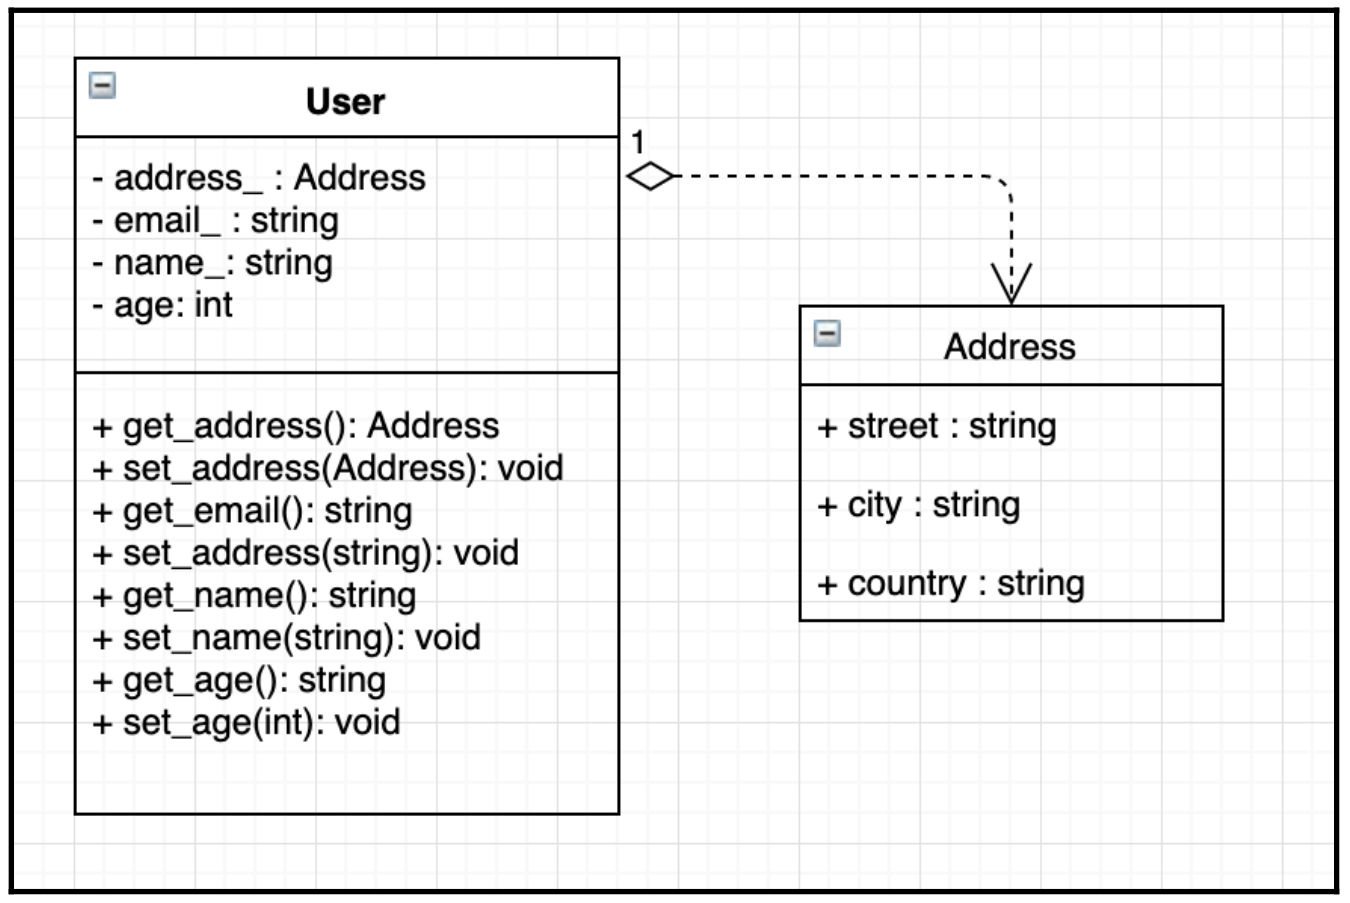
\includegraphics[width=0.8\textwidth]{content/Section-2/Chapter-10/6}
\end{center}

这些实体之间的关系将在设计过程中变得清晰。例如,地址本身不是一个实体,它是用户的一部分。也就是说,如果用户对象没有实例化,它就不能有实例。然而,正如我们可能希望指向可重用代码,地址类型也可以用于仓库对象。也就是说,用户和地址之间的关系是简单的聚合,而不是组合。 \par
在讨论支付选项时,我们可以对User类型提出更多要求。该平台的用户应该能够插入为产品付费的选项。在决定如何在User类中表示支付选项之前,应该找出这些选项到底是什么。简单起见,假设支付选项包含信用卡号、持卡人姓名、到期日期和卡的安全码。这听起来像是另一种数据聚合,所以让我们将所有这些都收集到一个结构中,如下所示: \par

\begin{lstlisting}[caption={}]
struct PaymentOption
{
	std::string number;
	std::string holder_name;
	std::chrono::year_month expiration_date;
	int code;
};
\end{lstlisting}

注意std::chrono::year\underline{ }month在前面的结构体中,表示特定年份的特定月份(C++20)。大多数支付卡只携带卡过期的月份和年份,所以这个std::chrono::year\underline{ }month功能对于PaymentOption是完美的。 \par
因此,在设计用户类的过程中,我们提出了一个新的类型——PaymentOption。一个用户可以有多个支付选项,因此User和PaymentOption之间的关系是一对多。现在让我们用这个新的聚合来更新我们的用户类图(这个例子中我们使用的是复合): \par

\begin{center}
	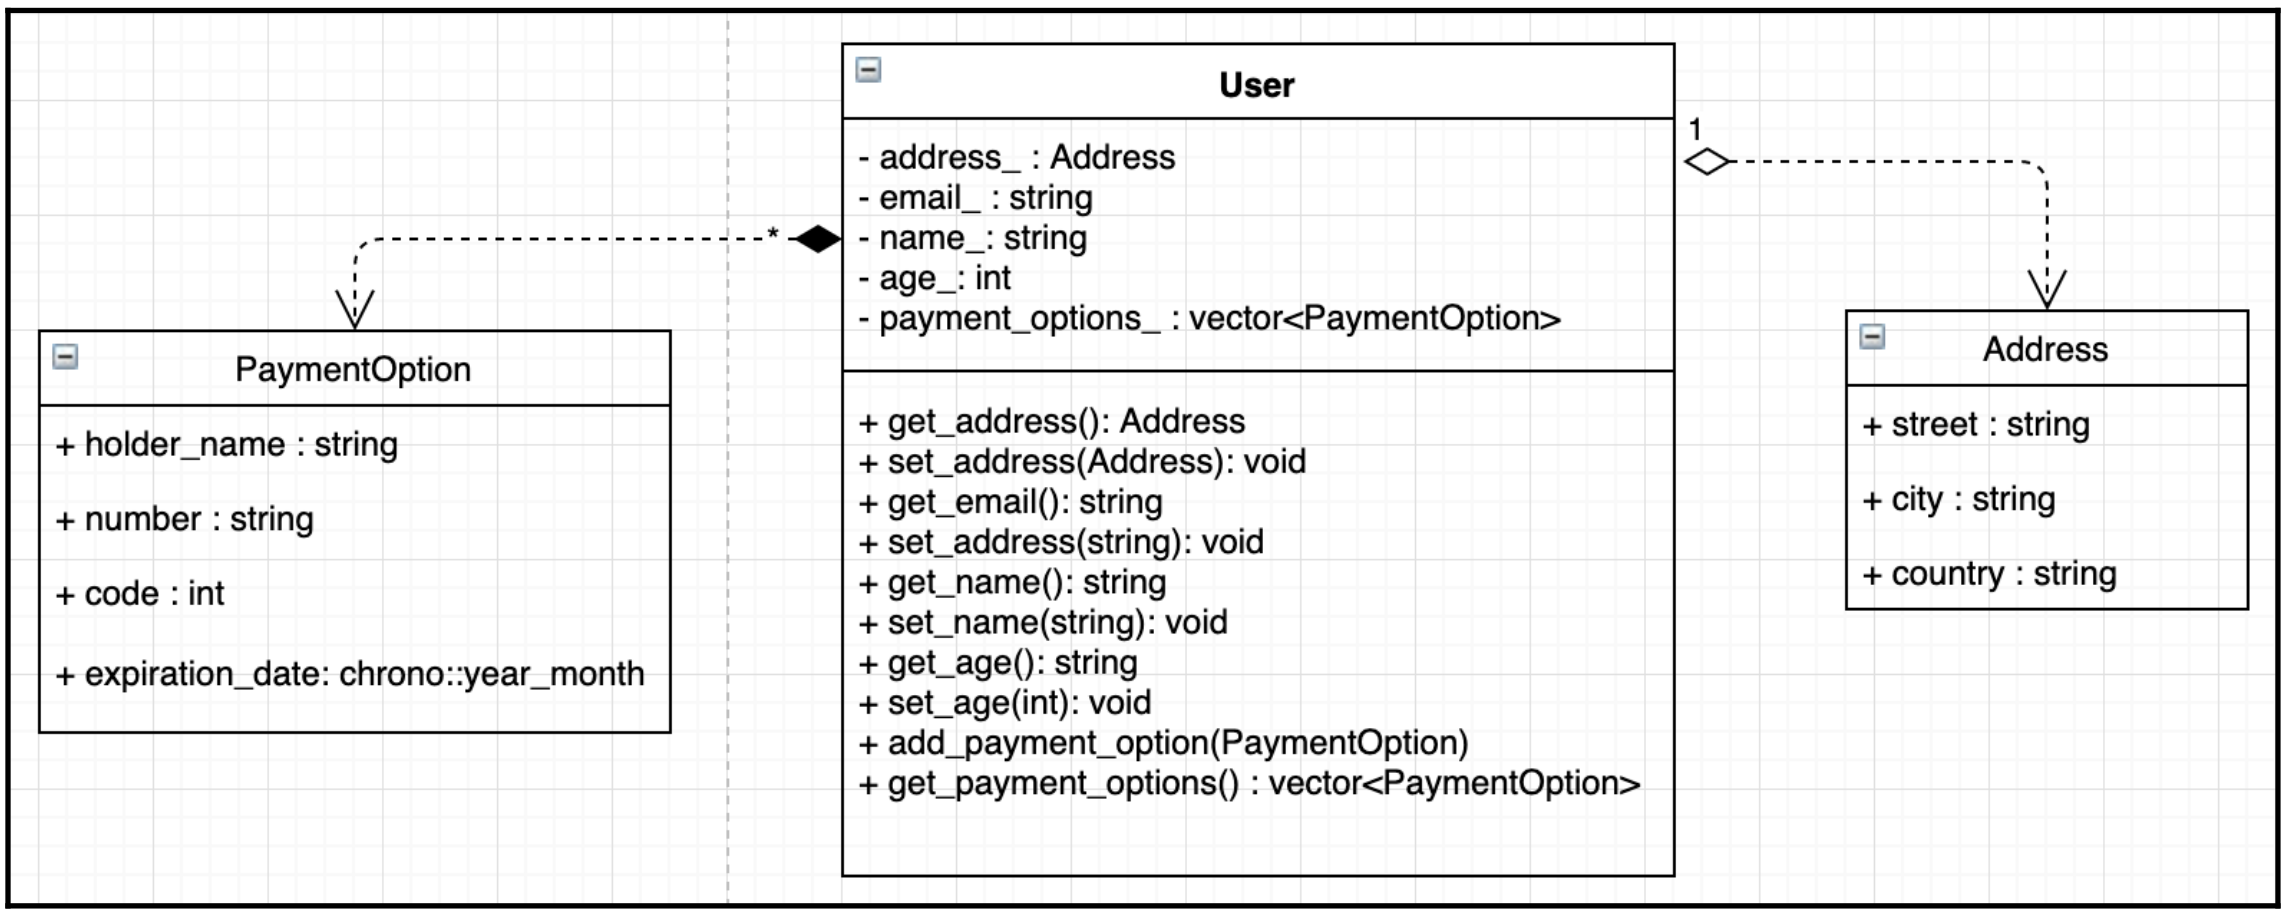
\includegraphics[width=1.\textwidth]{content/Section-2/Chapter-10/7}
\end{center}

User和PaymentOption之间的依赖关系如下代码所示: \par

\begin{lstlisting}[caption={}]
class User
{
public:
	// code omitted for brevity
	void add_payment_option(const PaymentOption& po) {
		payment_options_.push_back(op);
	}
	std::vector get_payment_options() const {
		return payment_options_;
	}
private:
	// code omitted for brevity
	std::vector<PaymentOption> payment_options_;
};
\end{lstlisting}

即使用户可能设置了多个支付选项,我们也应该将其中一个标记为主要支付选项。这很棘手,因为我们可以将所有选项存储在vector中,但现在我们必须将其中一个选项作为主选项。 \par
我们可以使用pair或tuple(如果比较花哨的话),将vector中的选项映射为布尔值,以指示它是否是主值。下面的代码描述了前面介绍的User类中tuple的用法: \par

\begin{lstlisting}[caption={}]
class User
{
public:
	// code omitted for brevity
	void add_payment_option(const PaymentOption& po, bool is_primary) {
		payment_options_.push_back(std::make_tuple(po, is_primary));
	}

	std::vector<std::tuple<PaymentOption, boolean> > get_payment_options()
	const {
		return payment_options_;
	}
private:
	// code omitted for brevity
	std::vector<std::tuple<PaymentOption, boolean> > payment_options_;
};
\end{lstlisting}

我们可以通过以下方式,利用类型别名来简化代码: \par

\begin{lstlisting}[caption={}]
class User
{
public:
	// code omitted for brevity
	using PaymentOptionList = std::vector<std::tuple<PaymentOption, boolean>
	>;
	
	// add_payment_option is omitted for brevity
	PaymentOptionList get_payment_options() const {
		return payment_options_;
	}

private:
	// code omitted for brevity
	PaymentOptionList payment_options_;
};
\end{lstlisting}

下面是User类如何检索用户的主要支付选项: \par

\begin{lstlisting}[caption={}]
User john = get_current_user(); // consider the function is implemented and works
auto payment_options = john.get_payment_options();
for (const auto& option : payment_options) {
	auto [po, is_primary] = option;
	if (is_primary) {
		// use the po payment option
	}
}
\end{lstlisting}

我们在访问for循环中的元组项时使用了结构化绑定。然而,在学习了关于数据结构和算法的章节之后,现在意识到搜索主要支付选项是一个线性操作。每次我们需要检索主要支付选项时都要遍历vector,这可能是一种糟糕的做法。 \par

\hspace*{\fill} \\ %插入空行

\includegraphics[width=0.05\textwidth]{images/tip}
您可以更改底层的数据结构,以提高运行速度。元素的访问是常量时间复杂度时,速度会变得更快。在这个场景中,我们应该将一个布尔值映射为支付选项。对于除一个选项外的所有选项,布尔值都是相同的值。它将导致哈希冲突,这种冲突将通过将映射到相同散列表值的值链接在一起来处理。使用哈希表的唯一好处是对主要支付选项的固定时间访问。 \par
\noindent\textbf{}\ \par

最后,我们给出了在类中单独存储主要支付选项的最简单的解决方案。以下,是我们应该如何重写用户类中的支付选项处理部分: \par

\begin{lstlisting}[caption={}]
class User
{
public:
	// code omitted for brevity
	using PaymentOptionList = std::vector<PaymentOption>;
	PaymentOption get_primary_payment_option() const {
		return primary_payment_option_;
	}

	PaymentOptionList get_payment_options() const {
		return payment_options_;
	}

	void add_payment_option(const PaymentOption& po, bool is_primary) {
		if (is_primary) {
			// moving current primary option to non-primaries
			add_payment_option(primary_payment_option_, false);
			primary_payment_option_ = po;
			return;
		}
		payment_options_.push_back(po);
	}

private:
	// code omitted for brevity
	PaymentOption primary_payment_option_;
	PaymentOptionList payment_options_;
};
\end{lstlisting}

目前为止,我们经历了定义存储支付选项的方法的过程,只是为了展示编码之前的设计过程。虽然我们已经为单一情况下的支付选项创造了许多版本,但都不是最终版本。在支付选项向量中总是存在处理重复值的情况。当向用户添加一个支付选项作为主要选项,然后再添加另一个选项作为主要选项时,前一个选项将进入非主要列表。如果我们改变主意,再次将旧的支付选项添加为主要选项,其不会从非主要选项列表中删除。 \par
所以,总有机会深入思考,避免潜在的问题。设计和编码是相辅相成的,也别忘了TDD。大多数情况下,在编写代码之前编写测试将帮助您发现许多问题。 \par

\noindent\textbf{}\ \par
\textbf{使用SOLID原则} \ \par
有很多原则和设计方法可以在项目设计中使用。保持设计简单是最好的,然而,有一些原则在几乎所有项目中都是有用的。例如,SOLID由5个原则组成,其中的全部或部分原则可能对设计有用。 \par
SOLID代表以下原则: \par

\begin{itemize}
	\item 单一责任原则
	\item 开闭原则
	\item 里氏替换原则
	\item 接口分离原则
	\item 依赖倒置原则
\end{itemize}

让我们结合例子来讨论下每个原则。

\noindent\textbf{}\ \par
\textbf{单一责任原则} \ \par
单一责任原则强调简单,即一个对象一项任务。尽量减少对象功能关系的复杂性。让每个对象都有一个职责,不过把一个复杂的对象分解成更小更简单的组件并不总是那么容易。单一责任是一个上下文绑定的概念,不是关于在一个类中只有一个方法,而是关于让类或模块负责一件事。例如,我们前面设计的User类有一个职责:存储用户信息。然而,我们在User类中添加了支付选项,并强制它具有添加和删除支付选项的方法。我们还引入了一个主要的支付选项,它在用户方法中包含了额外的逻辑。 \par
第一个建议将User类分解为两个单独的类。每个类都有一个单独的职责。下面的类图描述了这个想法: \par

\begin{center}
	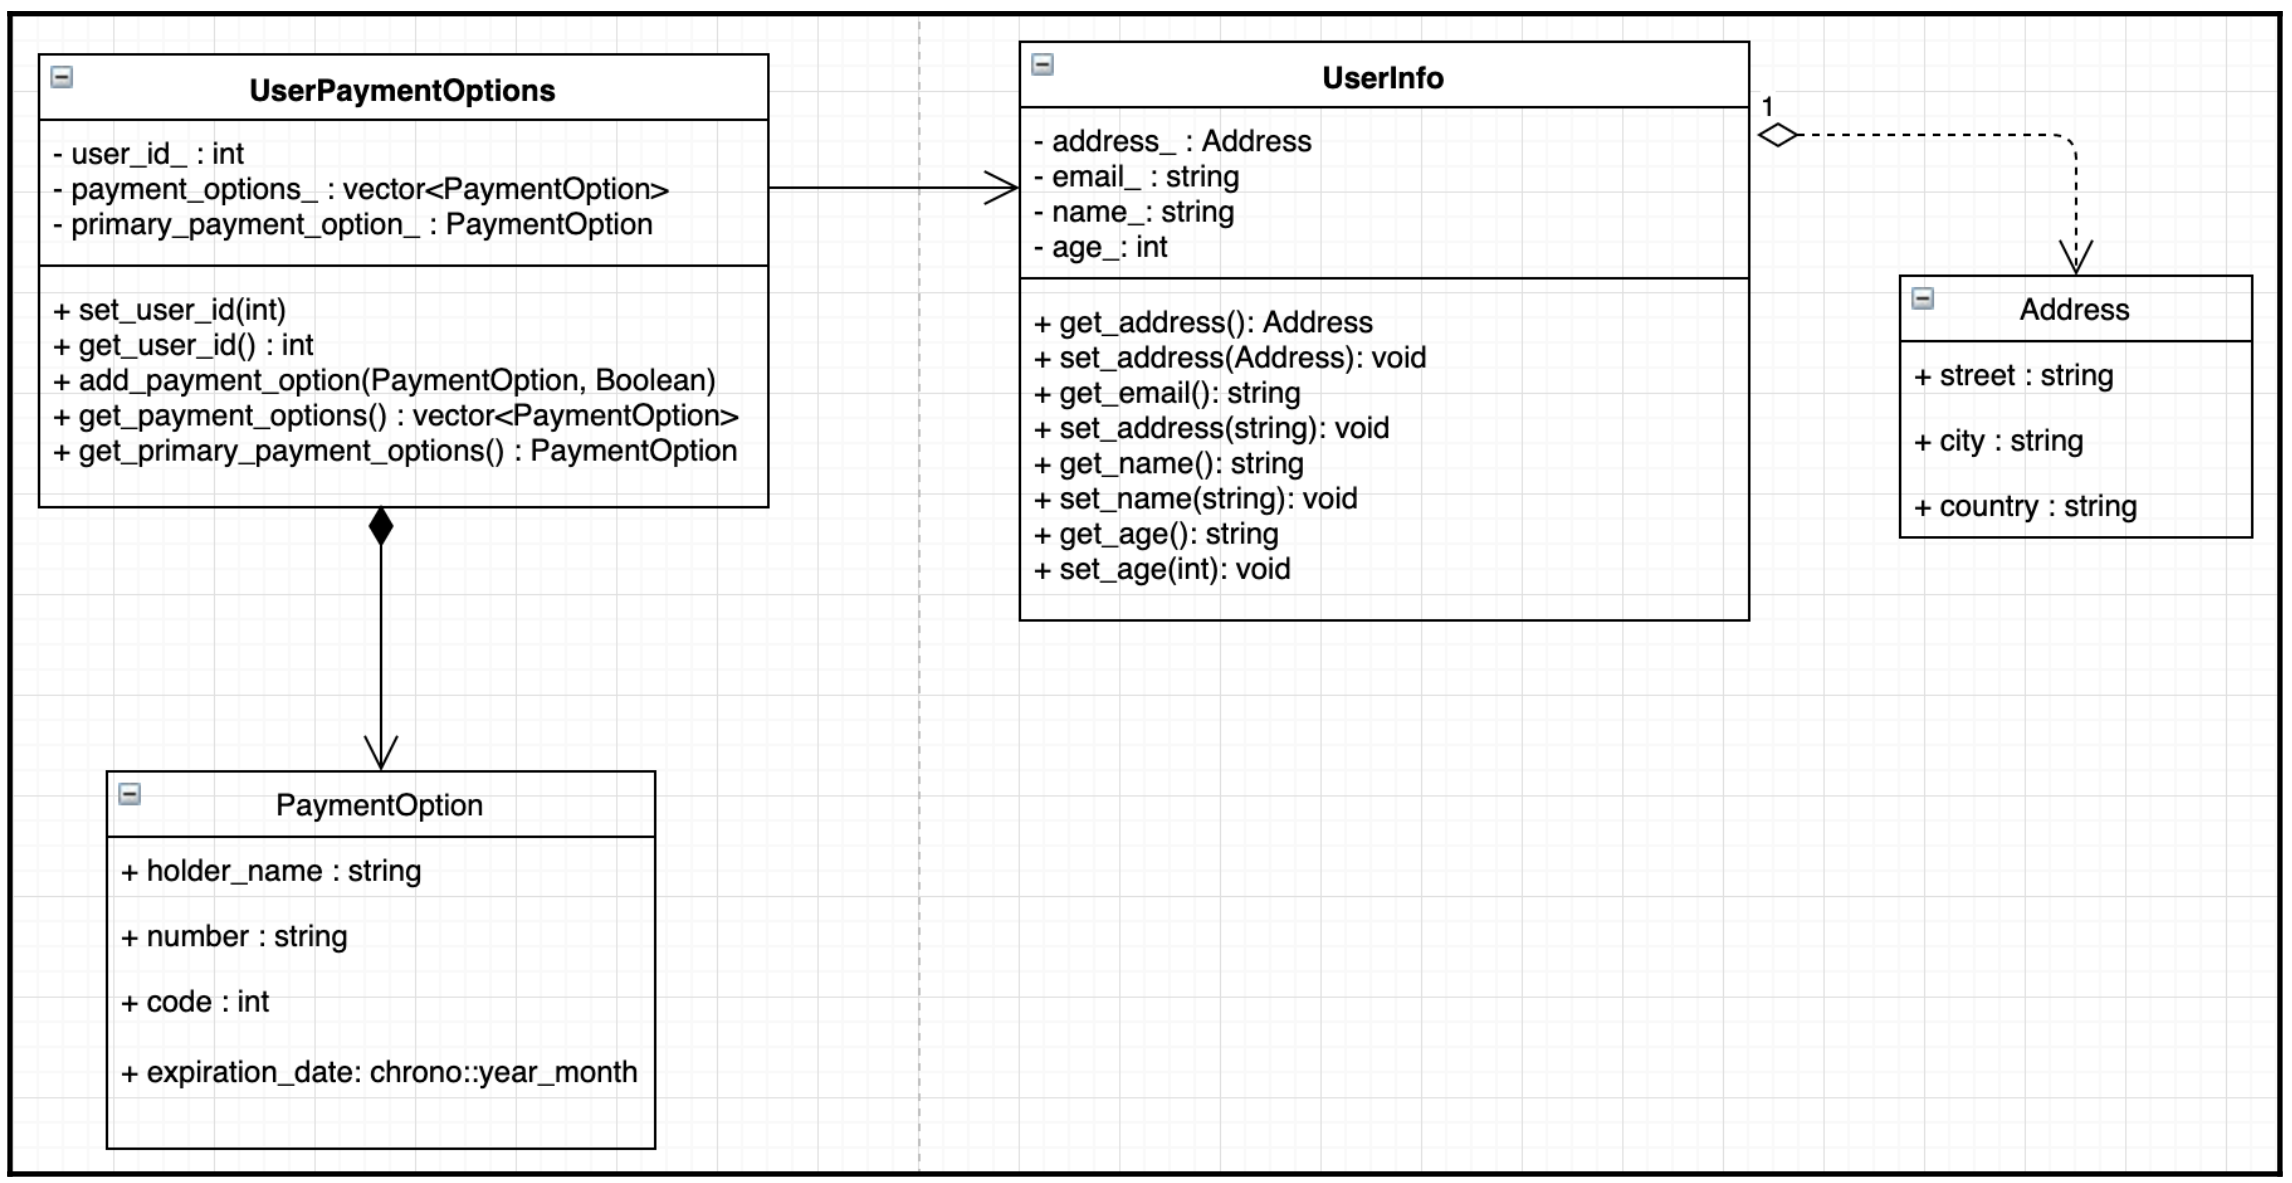
\includegraphics[width=1.\textwidth]{content/Section-2/Chapter-10/8}
\end{center}

其中一个将只存储用户的基本信息,下一个将存储用户的支付选项。我们将它们命名为UserInfo和UserPaymentOptions。有些人可能会喜欢这个新设计,但我们会坚持旧的设计。这是为什么呢?虽然User类包含用户信息和支付选项,但后者也表示一条信息。我们设置和获取支付选项的方式与设置和获取用户电子邮件的方式相同。因此,我们保持User类不变,因为它满足了单一职责原则。当我们在User类中添加支付功能时,这将打破原始设计。在该场景中,User类将存储用户信息并进行支付事务。就单一责任原则而言,这是不可接受的,因此,我们不会这么做。 \par
单一责任原则也与职能有关。add\underline{ }payment\underline{ }option()方法有两个职责。如果函数的第二个(默认)参数为true,将添加一个新的主要支付选项。否则,会将新的支付选项添加到非主要选项列表中。最好有一个单独的方法来添加一个主要的支付选项。这样,每个方法都有一个单独的职责。 \par

\noindent\textbf{}\ \par
\textbf{开闭原则} \ \par
开闭原则是指类应该对扩展开放,但对修改关闭。这意味着当需要新的功能时,最好扩展基本功能,而不是修改。以设计的电子商务应用程序的Product类为例,下面是Product类的一个简单图: \par

\begin{center}
	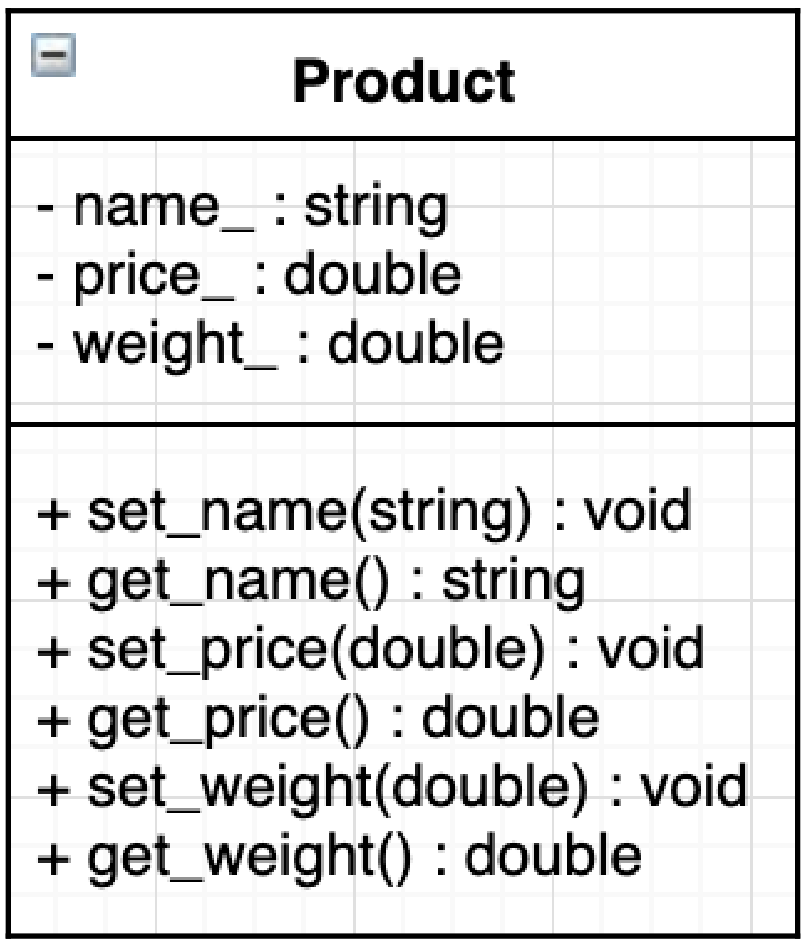
\includegraphics[width=0.4\textwidth]{content/Section-2/Chapter-10/9}
\end{center}

每个Product对象有三个属性:名称、价格和重量。想象一下,在设计了产品类和整个电子商务平台之后,来自客户的新需求。他们现在想买数字产品,如:电子书、电影和录音。除了产品的重量之外,一切都很好。现在可能有两种产品——有形的和数字的——我们应该重新思考产品使用的逻辑。我们可以在产品中加入一个新功能,如下代码所示: \par

\begin{lstlisting}[caption={}]
class Product
{
public:
	// code omitted for brevity
	bool is_digital() const {
		return weight_ == 0.0;
	}
	// code omitted for brevity
};
\end{lstlisting}

显然,我们修改了类,违背了开闭原则。这个原则是说这个类应该关闭以进行修改。它应该开放扩展。我们可以通过重新设计Product类并使其成为所有产品的抽象基类来实现这一点。接下来,我们创建另外两个继承Product基类的类:PhysicalProduct和DigitalProduct。下面的类图描述了新的设计: \par

\begin{center}
	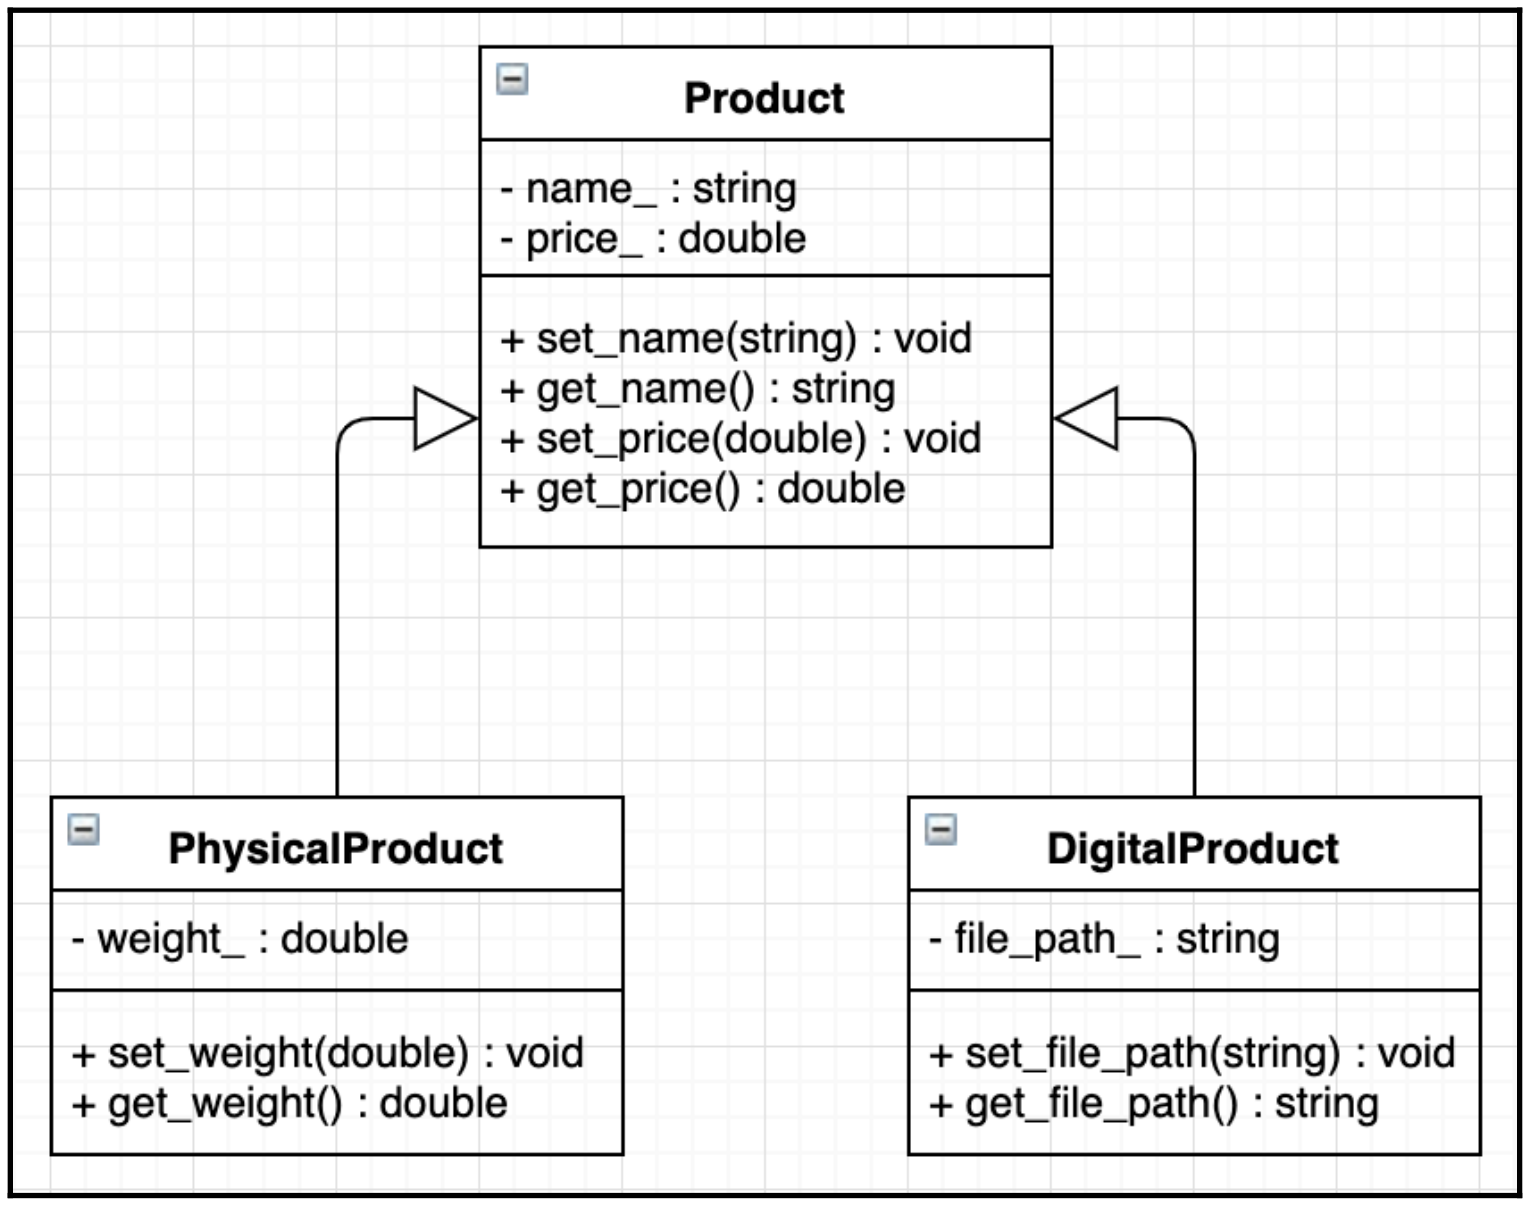
\includegraphics[width=0.6\textwidth]{content/Section-2/Chapter-10/10}
\end{center}

正如您在前面的图表中看到的,我们从Product类中删除了weight\underline{ }属性。现在我们又多了两个类,PhysicalProduct有一个weight\underline{ }property,而DigitalProduct没有。相反,其有一个file\underline{ }path\underline{ }属性。这种方法满足开闭原则,因为现在所有的类都可以扩展。我们使用继承来扩展类,下面的原则与之密切相关。 \par

\noindent\textbf{}\ \par
\textbf{里氏替换原则} \ \par
里氏替换原则是以正确的方式继承。简单地说,如果有函数接受某种类型的参数,那么这个函数应该接受派生类型的参数。 \par

\hspace*{\fill} \\ %插入空行

\includegraphics[width=0.05\textwidth]{images/warn}
里氏替代原理是以图灵奖得主、计算机科学博士Barbara Liskov的名字命名的。 \par
\noindent\textbf{}\ \par

当你理解了继承和里氏替换原理,你就很难忘记它。让我们继续开发Product类并添加一个新方法,该方法根据货币类型返回产品的价格。我们可以将价格存储在相同的货币单位中,并提供一个函数将价格转换为指定的货币。下面是该方法的简单实现: \par

\begin{lstlisting}[caption={}]
enum class Currency { USD, EUR, GBP }; // the list goes further

class Product
{
public:
	// code omitted for brevity
	double convert_price(Currency c) {
		// convert to proper value
	}

	// code omitted for brevity
};
\end{lstlisting}

过了一段时间,该公司决定纳入所有数字产品的终身折扣。现在,所有的数码产品都有12\%的优惠。我们在DigitalProduct类中添加了一个单独的函数,该函数通过应用折扣返回转换后的价格。下面是它在DigitalProduct中的样子: \par

\begin{lstlisting}[caption={}]
class DigitalProduct : public Product
{
public:
	// code omitted for brevity
	double convert_price_with_discount(Currency c) {
		// convert by applying a 12% discount
	}
};
\end{lstlisting}

设计上的问题显而易见。在DigitalProduct实例上调用convert\underline{ }price()不起作用。更糟糕的是,客户机代码不能调用它。它应该调用convert\underline{ }price\underline{ }with\underline{ }discount(),因为所有数字产品都必须以12\%的折扣销售。这种设计与里氏替换原理相矛盾。 \par
我们应该记住多态的美妙之处,而不是破坏类的层次结构。更好的版本应该是这样的: \par

\begin{lstlisting}[caption={}]
class Product
{
public:
	// code omitted for brevity
	virtual double convert_price(Currency c) {
		// default implementation
	}

	// code omitted for brevity
};

class DigitalProduct : public Product
{
public:
	// code omitted for brevity
	double convert_price(Currency c) override {
		// implementation applying a 12% discount
	}

	// code omitted for brevity
};
\end{lstlisting}

可以看到,我们不再需要convert\underline{ }price\underline{ }with\underline{ }discount()函数。里氏替换原则也成立。然而,我们应该再检查设计中的缺陷。让我们通过在基类中合并私有虚方法来计算折扣来改进它。以下更新版本的Product类包含一个名为calculate\underline{ }discount()的私有虚成员函数: \par

\begin{lstlisting}[caption={}]
class Product
{
public:
	// code omitted for brevity
	virtual double convert_price(Currency c) {
		auto final_price = apply_discount();
		// convert the final_price based on the currency
	}

private:
	virtual double apply_discount() {
		return getPrice(); // no discount by default
	}

	// code omitted for brevity
};
\end{lstlisting}

convert\underline{ }price()函数调用私有apply\underline{ }discount()函数,该函数按原样返回价格。在派生类中重写apply\underline{ }discount()函数,如下面的DigitalProduct实现所示: \par

\begin{lstlisting}[caption={}]
class DigitalProduct : public Product
{
public:
	// code omitted for brevity
private:
	double apply_discount() override {
		return getPrice() * 0.12;
	}
	// code omitted for brevity
};
\end{lstlisting}

我们不能在类之外调用私有函数,但可以在派生类中重写它。前面的代码展示了重写私有虚函数的优点。我们修改实现,保持接口不变。如果派生类不需要为折扣计算提供自定义功能,则不需要重写。另一方面,DigitalProduct在转换之前需要在价格上申请12\%的折扣。不需要修改基类的公共接口。 \par

\hspace*{\fill} \\ %插入空行

\includegraphics[width=0.05\textwidth]{images/warn}
应该考虑重新思考Product类的设计。因为总是返回最新的有效价格,所以在getPrice()中直接调用apply\underline{ }discount()似乎更好。 \par
\noindent\textbf{}\ \par

设计过程是创造性的。由于出现了意想不到的新需求,重写所有代码并不少见。我们使用原则和方法来最小化实现新功能后可能出现的破坏性更改。SOLID的下一个原则是使您的设计更加灵活的最佳实践。 \par

\noindent\textbf{}\ \par
\textbf{接口分离原则} \ \par
接口分离原则建议将复杂的接口划分为更简单的接口,这种分离允许类避免实现它们不使用的接口。 \par
在电子商务应用程序中,我们应该实现产品交付、替换和过期功能。产品的运输将产品项目移动到其买家(现阶段我们不关心装运细节)。更换产品考虑更换损坏或丢失的产品后,运输给买家。最后,让产品过期意味着扔掉那些在过期日期前没有销售的产品。 \par
我们可以自由地实现前面介绍的Product类中的所有功能。然而,我们会偶然发现一些类型的产品,例如:不能运输(例如,出售房子很少涉及运输给买家)。可能会有不可替代的产品。例如,一幅原画是不可能替代的,即使它丢失或损坏。最后,数字产品永远不会过期()大多数情况下是这样)。 \par
我们不应该强迫客户端代码实现它不需要的行为,指的是实现类的行为。下面的例子是一个不好的做法,与接口隔离原则相矛盾: \par

\begin{lstlisting}[caption={}]
class IShippableReplaceableExpirable
{
public:
	virtual void ship() = 0;
	virtual void replace() = 0;
	virtual void expire() = 0;
};
\end{lstlisting}

现在,Product类实现了前面所示的接口,必须为所有的方法提供一个实现。接口隔离原则提出以下模型: \par

\begin{lstlisting}[caption={}]
class IShippable
{
public:
	virtual void ship() = 0;
};
class IReplaceable
{
public:
	virtual void replace() = 0;
};
class IExpirable
{
public:
	virtual void expire() = 0;
};
\end{lstlisting}

现在,Product类跳过实现任何接口。它的派生类从特定类型派生(实现)。下面的示例声明了几种产品类,每种产品类都支持前面介绍的有限数量的行为。请注意,为了代码简洁,我们省略了类的主体: \par

\begin{lstlisting}[caption={}]
class PhysicalProduct : public Product {};
// The book does not expire
class Book : public PhysicalProduct, public IShippable, public IReplaceable
{
};

// A house is not shipped, not replaced, but it can expire
// if the landlord decided to put it on sell till a specified date
class House : public PhysicalProduct, public IExpirable
{
};

class DigitalProduct : public Product {};

// An audio book is not shippable and it cannot expire.
// But we implement IReplaceable in case we send a wrong file to the user.
class AudioBook : public DigitalProduct, public IReplaceable
{
};
\end{lstlisting}

如果您想打包一个下载的文件,请考虑为AudioBook实现IShippable。 \par

\noindent\textbf{}\ \par
\textbf{依赖倒置原则} \ \par
最后,依赖倒置表明对象不应该强耦合,允许轻松地切换到另一个依赖项。例如,当用户购买一个产品时,我们发送一个关于购买的收据。从技术上讲,发送收据有几种方式,即通过邮件打印发送,通过电子邮件发送,或在平台的用户账户页面上显示收据。对于后者,我们通过电子邮件或应用程序向用户发送通知,告诉他们收据已经可以查看了。看看下面打印收据的接口: \par

\begin{lstlisting}[caption={}]
class IReceiptSender
{
public:
	virtual void send_receipt() = 0;
};
\end{lstlisting}

让我们假设我们已经实现了Product类中的purchase()方法。完成后,我们发送收据。下面的代码发送了收据: \par

\begin{lstlisting}[caption={}]
class Product
{
public:
	// code omitted for brevity
	void purchase(IReceiptSender* receipt_sender) {
		// purchase logic omitted
		// we send the receipt passing purchase information
		receipt_sender->send(/* purchase-information */);
	}
};
\end{lstlisting}

我们可以根据需要添加尽可能多的收据打印选项来扩展应用程序。下面的类实现了IReceiptSender接口: \par

\begin{lstlisting}[caption={}]
class MailReceiptSender : public IReceiptSender
{
public:
	// code omitted for brevity
	void send_receipt() override { /* ... */ }
};
\end{lstlisting}

另外两个类——EmailReceiptSender和InAppReceiptSender——都实现了IReceiptSender。因此,要使用特定的收据,我们只需通过purchase()方法将依赖注入到Product类当中,如下所示: \par

\begin{lstlisting}[caption={}]
IReceiptSender* rs = new EmailReceiptSender();
// consider the get_purchasable_product() is implemented somewhere in the code
auto product = get_purchasable_product();
product.purchase(rs);
\end{lstlisting}

我们可以更进一步,在User类中实现一个方法,返回具体用户想要的收据发送选项。这将使类更加解耦。 \par
前面讨论的所有SOLID原则是一个自然的方式组合类。并不是必须要坚持这些原则,但它将会改进你的设计。 \par

\noindent\textbf{}\ \par
\textbf{使用域驱动的设计} \ \par
域是程序的主区域。我们正在讨论和设计一个以电子商务为主要概念,领域为电子商务平台。我们建议您在项目中考虑领域驱动设计。然而,这种方法也并不是程序设计的灵丹妙药。 \par
为了方便设计项目,有以下三层架构: \par

\begin{itemize}
	\item 业务描述
	\item 业务逻辑
	\item 业务数据
\end{itemize}

三层架构适用于客户端-服务器软件,就像我们在本章设计的那样。表述层向用户提供与产品、购买和运输相关的信息。它通过将结果输出到客户端来与其他层进行通信。它是客户端可以直接访问的层,例如:web浏览器。 \par
业务逻辑关心应用程序的功能。例如,用户浏览表示层提供的产品,并决定购买其中之一。处理请求是业务层的任务。在领域驱动的设计中,我们倾向于结合领域的实体,其属性可用来解决应用程序的复杂性。我们将用户作为User类的实例处理,将产品作为Product类的实例处理,以此类推。业务逻辑将购买产品的用户解释为创建Order对象的用户对象,而Order对象又与Product对象相关。然后,将Order对象绑定到与购买该产品相关的事务对象。购买的相应结果通过表述层表示。 \par
最后,数据层处理数据的存储和检索。从用户身份验证到产品购买,每个步骤都是从系统数据库检索或记录在系统数据库。 \par
将应用程序划分为几个层可以处理复杂性,编写具有单一职责的对象要好得多。领域驱动设计将实体与没有概念标识的对象区分开来,后者称为对象。例如,用户不区分每个事务,他们只关心事务所代表的信息。另一方面,User对象具有User类(实体)形式的标识。 \par
使用其他对象(或不使用)的对象上允许的操作,称为命名服务。服务是一种不绑定到特定对象的操作,例如:通过set\underline{ }name()方法设置用户名是不应该视为服务的操作。另一方面,用户购买产品是一种由服务封装的操作。 \par
最后,领域驱动的设计集成了存储库和工厂模式。存储库模式负责检索和存储域对象的方法,工厂模式创建域对象。使用这些模式允许在需要的时候交换替代的实现。现在,让我们来看看电子商务平台中设计模式的威力。 \par

\noindent\textbf{}\ \par
\textbf{利用设计模式} \ \par
设计模式是软件设计中的体系结构解决方案。需要注意的是,设计模式既不是方法,也不是算法。它们是一种体系结构构造,提供了一种组织类及其关系的方法,以便在代码可维护性方面获得更好的结果。即使以前没有使用过一个设计模式,在软件设计中许多问题往往会重复出现。例如,为现有库创建更好的接口是一种称为Facade模式。设计模式有名称,以便开发者在对话或文档中使用。您应该很自然地与使用Facade模式、工厂模式等的其他开发者沟通。 \par
我们前面已经提到过,域驱动的设计合并了存储库和工厂模式。现在让我们来看看它们是什么,以及它们在我们的设计工作中有什么用处。 \par

\noindent\textbf{}\ \par
\textbf{库模式} \ \par
正如Martin Fowler所描述的那样,存储库模式“使用一个用于访问域对象的类集成接口在域层和数据映射层间充当中介”。 \par
该模式为数据操作提供了简单的方法,不需要直接使用数据库驱动程序。添加、更新、删除或选择适合应用程序域。 \par
其中一种方法是创建提供必要函数的通用存储库类。简单接口如下: \par

\begin{lstlisting}[caption={}]
class Entity; // new base class

template <typename T, typename = std::enable_if_t<std::is_base_of_v<Entity,
T>>>
class Repository
{
	public:
	T get_by_id(int);
	void insert(const T&);
	void update(const T&);
	void remove(const T&);
	std::vector<T> get_all(std::function<bool(T)> condition);
};
\end{lstlisting}

我们引入了一个名为Entity的新类。Repository类处理实体,并确保每个实体都符合实体的相同接口,将std::enable\underline{ }if和std::is\underline{ }base\underline{ }of\underline{ }v应用到模板参数中。 \par

\hspace*{\fill} \\ %插入空行

\includegraphics[width=0.05\textwidth]{images/warn}
std::is\underline{ }base\underline{ }of\underline{ }v是std::is\underline{ }base\underline{ }of<>::value的简短表示。\\同样,std::enable\underline{ }if\underline{ }t替换了std::enable\underline{ }if<>::type。 \par
\noindent\textbf{}\ \par

Entity类就像下面这样简单: \par

\begin{lstlisting}[caption={}]
class Entity
{
public:
	int get_id() const;
	void set_id(int);
private:
	int id_;
};
\end{lstlisting}

每个业务对象都是一个实体。因此,前面讨论的类应该更新为从Entity继承。例如,User类采用以下形式: \par

\begin{lstlisting}[caption={}]
class User : public Entity
{
	// code omitted for brevity
};
\end{lstlisting}

因此,我们可以用以下方式来使用存储库: \par

\begin{lstlisting}[caption={}]
Repository<User> user_repo;
User fetched_user = user_repo.get_by_id(111);
\end{lstlisting}

前面的存储库模式只是对这个主题的简单介绍,但可以使它更加强大。尽管使用Facade模式的重点不是访问数据库,但仍然可以用这个示例来解释它。Facade模式包装了一个或多个复杂的类,为客户机提供了预定义接口来处理底层功能。 \par

\noindent\textbf{}\ \par
\textbf{工厂模式} \ \par
当开发者谈论工厂模式时,他们可能会混淆工厂方法和抽象工厂模式,这两种创建模式都提供了各种创建机制。让我们讨论一下工厂的方法。它提供了一个在基类中创建对象的接口,并允许派生类修改将要创建的对象。 \par
现在是处理物流的时候了,工厂方法会帮助我们。当开发一个提供产品发货的电子商务平台时,应该考虑到并非所有用户都居住在仓库所在的同一区域。所以,将产品从仓库运送给买家,你应该选择合适的运输方式,自行车、无人机、卡车等。设计一个灵活的物流管理系统是研究的重点。 \par
不同的运输方式需要不同的实现。然而,它们都符合一个接口。以下是传输接口及其派生的特定传输实现类图: \par

\begin{center}
	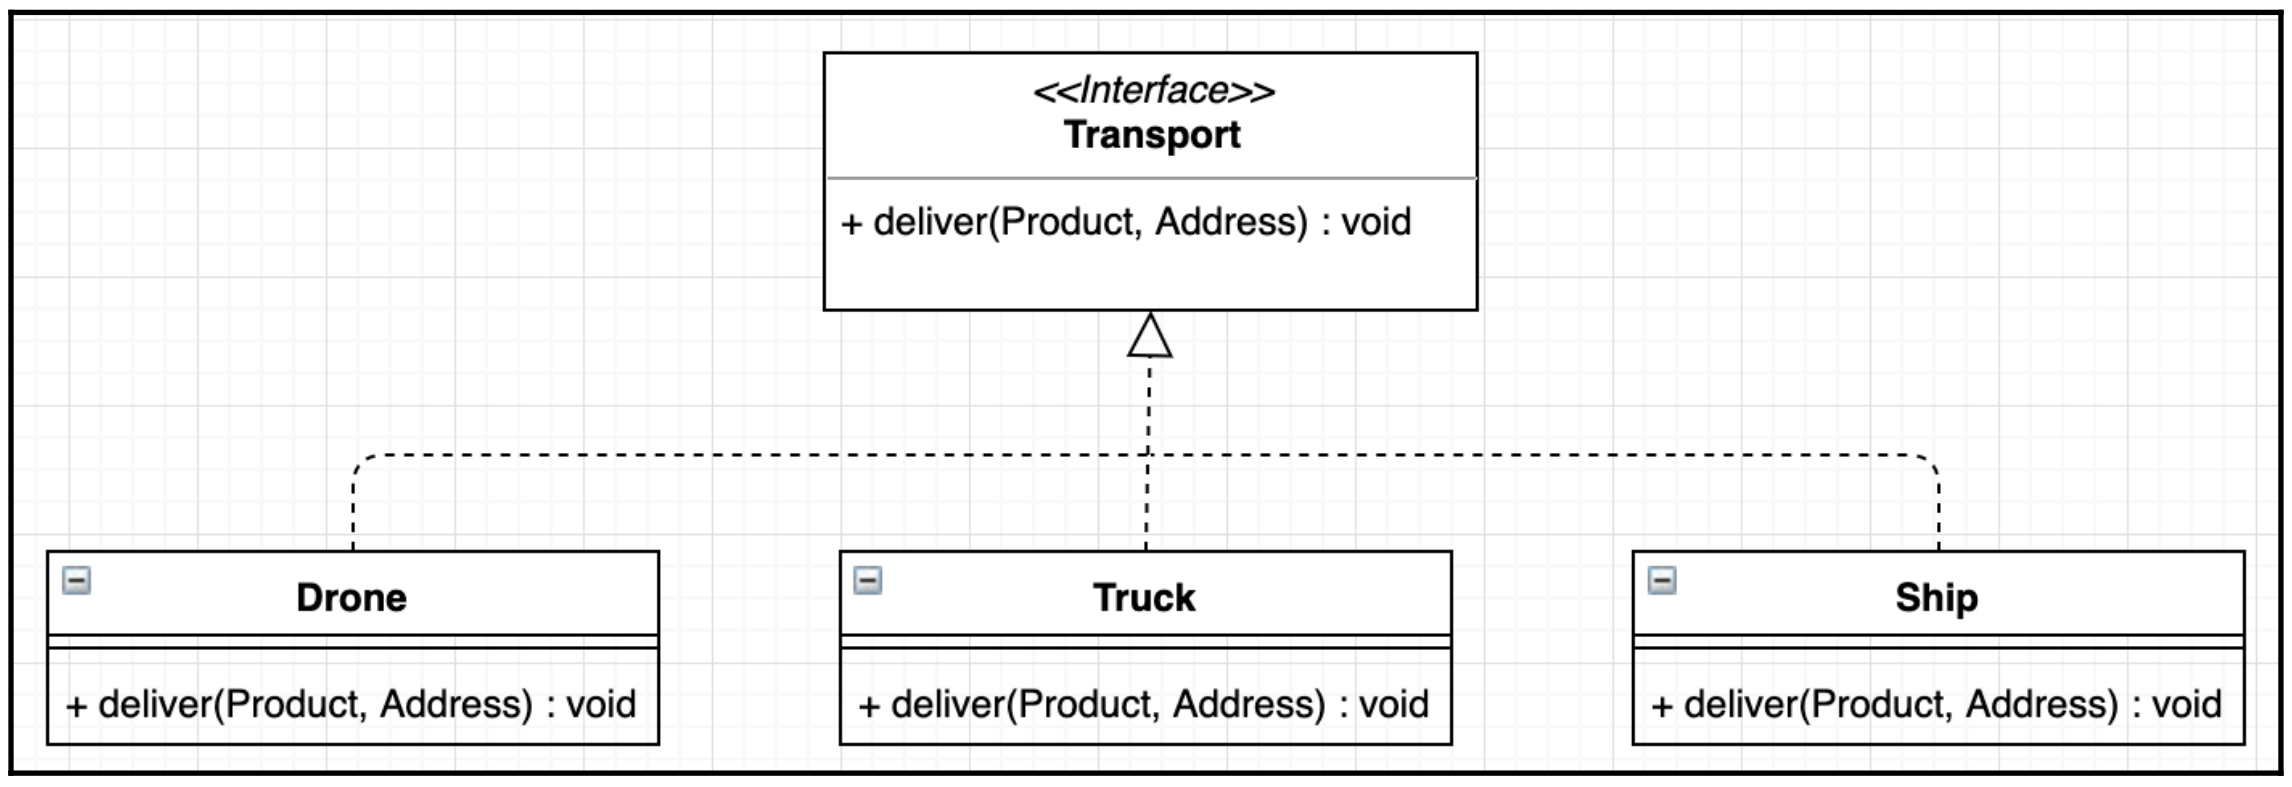
\includegraphics[width=0.8\textwidth]{content/Section-2/Chapter-10/11}
\end{center}

上图中的每个具体类都提供了交付的具体实现。 \par
假设我们设计了以下物流基类,负责与物流相关的行动,包括选择合适的运输方式,如下图所示: \par

\begin{center}
	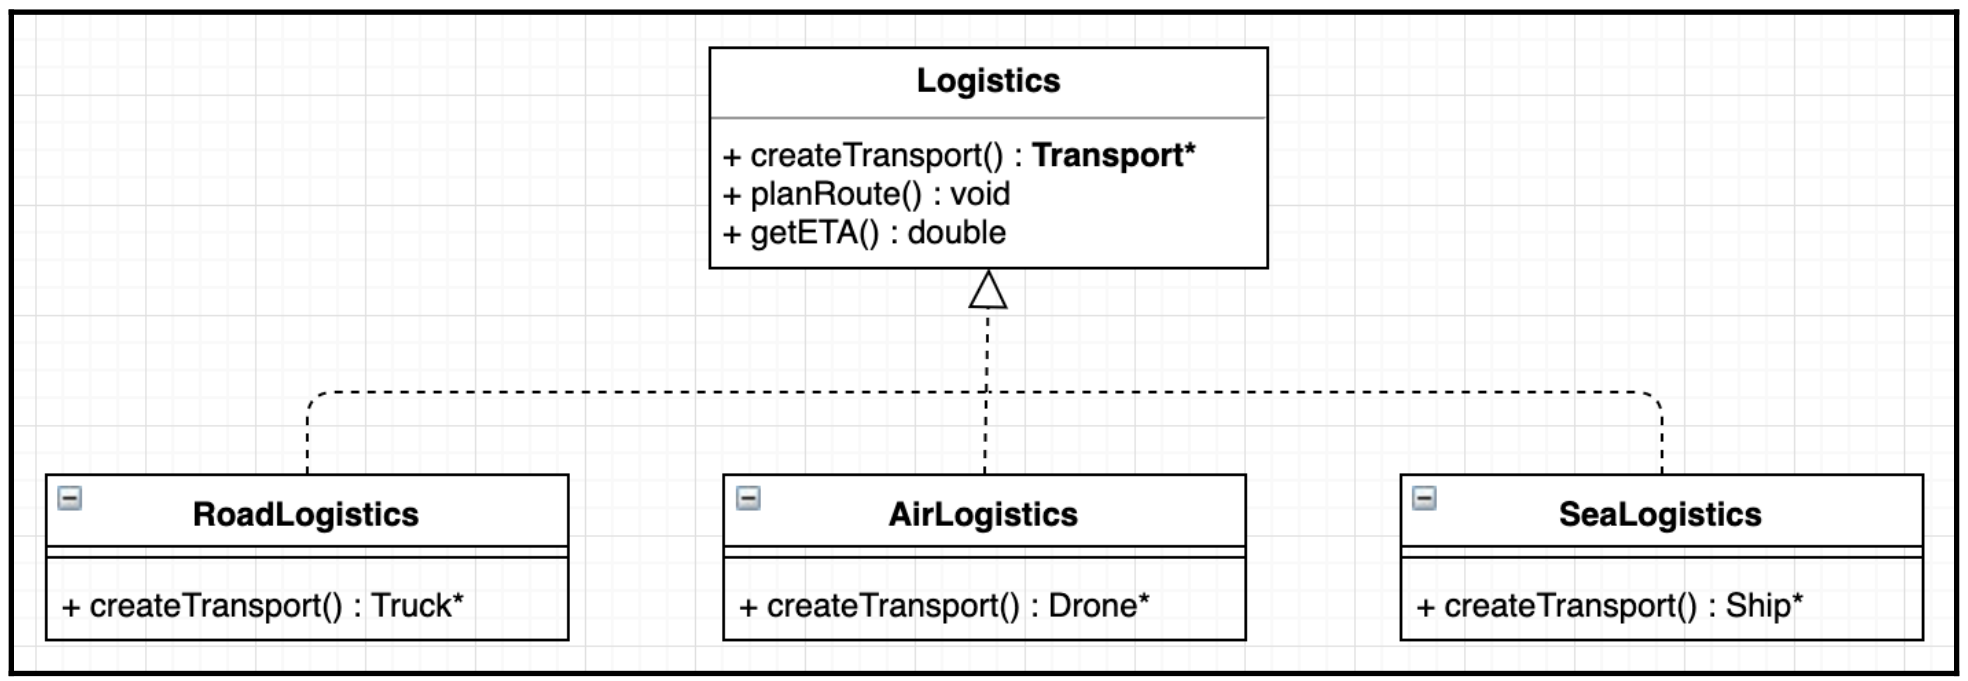
\includegraphics[width=0.8\textwidth]{content/Section-2/Chapter-10/12}
\end{center}

前面应用的工厂方法允许增加新的运输类型和新的物流方法。请注意createTransport()方法,它返回一个指向Transport的指针。派生类覆盖该方法,每个派生类都返回Transport的子类,因此提供了特定的传输模式,否则,我们不能在重写基类方法时返回不同的类型。 \par
物流中的createTransport()如下所示: \par

\begin{lstlisting}[caption={}]
class Logistics
{
	public:
	Transport* getLogistics() = 0;
	// other functions are omitted for brevity
};
\end{lstlisting}

Transport类表示无人机、卡车和船舶的基类。这意味着我们可以为它们创建一个实例,并使用一个Transport指针来引用它们,如下所示: \par

\begin{lstlisting}[caption={}]
Transport* ship_transport = new Ship();
\end{lstlisting}

这是工厂模式的基础,因为RoadLogistics,例如:复写getLogistics(): \par

\begin{lstlisting}[caption={}]
class RoadLogistics : public Logistics
{
public:
	Truck* getLogistics() override {
		return new Truck();
	}
}
\end{lstlisting}

注意函数的返回类型,它是Truck而不是Transport。它能起作用是因为卡车继承了Transport。另外,还可以看到对象创建是如何与对象本身解耦的。创建新对象通过工厂完成,这与前面讨论的SOLID原则保持一致。 \par
乍一看,利用设计模式将额外的复杂性合并到设计中,这可能令人困惑。然而,在实践设计模式时,应该具有更好的设计,因为允许项目的灵活性和可扩展性。 \par

\noindent\textbf{}\ \par
\textbf{总结} \ \par
软件开发需要细致的规划和设计。本章中,我们了解到项目开发包括以下步骤: \par

\begin{itemize}
	\item 需求收集和分析:了解项目的领域,讨论并确定应该实现的特性。
	\item 创建规则说明:记录需求和项目功能。
	\item 设计和测试计划:指从较大的实体开始设计项目,将每个实体分解为与项目中的其他类相关的单独的类。这一步还包括计划如何测试项目。
	\item 编码:此步骤涉及编写代码,以实现前面步骤中指定的项目。
	\item 测试和稳定性:根据预先计划的用例和场景检查项目,以发现问题并修复它们。
	\item 发布和维护:项目发布和维护是最后一步。
\end{itemize}

项目设计对开发者来说是一项复杂的任务。他们应该提前考虑,因为部分特性是在开发过程中引入的。 \par
为了使设计更灵活和健壮,我们讨论了更好架构的原则和模式。我们已经了解了设计一个复杂软件项目的过程。 \par
避免糟糕设计决策的最佳方法之一是,遵循已经设计好的模式和实践。应该考虑在未来的项目中,使用可靠的原则和经过验证的设计模式。 \par
下一章中,我们将设计一款策略游戏。将熟悉的设计模式进行应用,并看到它们如何出现在游戏开发中。 \par

\noindent\textbf{}\ \par
\textbf{问题} \ \par
\begin{enumerate}
	\item TDD的好处是什么?
	\item UML中交互图的目的是什么?
	\item 合成和聚合有什么区别?
	\item 如何描述里氏替换原则?
	\item 让我们假设给您一个类Animal和一个类Monkey。后者描述的是一种特殊的在树上跳的动物。从动物类继承猴子类是否违背开闭原则?
	\item 在本章的Product类及其子类上应用工厂模式。
\end{enumerate}

\noindent\textbf{}\ \par
\textbf{扩展阅读} \ \par
更多资料请参阅: \par
\begin{itemize}
	\item Object-Oriented Analysis and Design with Applications by Grady Booch,  https:/​/www.​amazon.​com/​Object-​Oriented-​Analysis-​Design-​Applications-​3rd/​dp/	020189551X/​
	\item Design Patterns: Elements of Reusable Object-Oriented Software by Erich Gamma et	al, https:/​/​www.​amazon.​com/​Design-​Patterns-​Elements-​Reusable-​Object-	Oriented/​dp/​0201633612/​
	\item Code Complete: A Practical Handbook of Software Construction by Steve McConnel, https://www.amazon.com/Code-Complete-Practical-Handbook-Construction/dp/0735619670/
	\item Domain-Driven Design: Tackling Complexity in the Heart of Software by Eric	Evans,  https:/​/​www.​amazon.​com/​Domain-​Driven-​Design-​Tackling-
	Complexity-​Software/​dp/​0321125215/
\end{itemize}

\newpage










